% Chapter 3: Efficient Market Hypothesis
% Harvard-quality academic presentation
% Bachelor program, Bucharest University of Economic Studies

\documentclass[9pt, aspectratio=169, t]{beamer}

% Ensure content fits on slides
\setbeamersize{text margin left=8mm, text margin right=8mm}

%=============================================================================
% THEME AND STYLE CONFIGURATION
%=============================================================================
\usetheme{default}

% Color Palette
\definecolor{MainBlue}{RGB}{26, 58, 110}
\definecolor{AccentBlue}{RGB}{26, 58, 110}
\definecolor{IDAred}{RGB}{205, 0, 0}
\definecolor{DarkGray}{RGB}{51, 51, 51}
\definecolor{MediumGray}{RGB}{128, 128, 128}
\definecolor{LightGray}{RGB}{248, 248, 248}
\definecolor{VeryLightGray}{RGB}{235, 235, 235}
\definecolor{KeynoteGray}{RGB}{218, 218, 218}
\definecolor{SectionGray}{RGB}{120, 120, 120}
\definecolor{FooterGray}{RGB}{100, 100, 100}
\definecolor{Crimson}{RGB}{220, 53, 69}
\definecolor{Forest}{RGB}{46, 125, 50}
\definecolor{Amber}{RGB}{181, 133, 63}
\definecolor{Orange}{RGB}{230, 126, 34}
\definecolor{Purple}{RGB}{142, 68, 173}

% Gradient background (exact Keynote 315° gradient: white to RGB 218,218,218)
\setbeamertemplate{background}{%
    \begin{tikzpicture}[remember picture, overlay]
        \shade[shading=axis, shading angle=315,
        top color=white, bottom color=KeynoteGray]
        (current page.south west) rectangle (current page.north east);
    \end{tikzpicture}%
}
\setbeamercolor{background canvas}{bg=}

\setbeamercolor{palette primary}{bg=MainBlue, fg=white}
\setbeamercolor{palette secondary}{bg=MainBlue!85, fg=white}
\setbeamercolor{palette tertiary}{bg=MainBlue!70, fg=white}
\setbeamercolor{structure}{fg=MainBlue}
\setbeamercolor{title}{fg=IDAred}
\setbeamercolor{frametitle}{fg=IDAred, bg=}
\setbeamercolor{block title}{bg=MainBlue, fg=white}
\setbeamercolor{block body}{bg=VeryLightGray, fg=DarkGray}
\setbeamercolor{block title alerted}{bg=Crimson, fg=white}
\setbeamercolor{block body alerted}{bg=Crimson!8, fg=DarkGray}
\setbeamercolor{block title example}{bg=Forest, fg=white}
\setbeamercolor{block body example}{bg=Forest!8, fg=DarkGray}
\setbeamercolor{item}{fg=MainBlue}

\setbeamercolor{author in head/foot}{fg=FooterGray, bg=}
\setbeamercolor{title in head/foot}{fg=FooterGray, bg=}
\setbeamercolor{date in head/foot}{fg=FooterGray, bg=}
\setbeamercolor{section in head/foot}{fg=FooterGray, bg=}
\setbeamercolor{subsection in head/foot}{fg=FooterGray, bg=}

\setbeamertemplate{itemize item}{\color{MainBlue}$\boxdot$}
\setbeamertemplate{itemize subitem}{\color{MainBlue}$\blacktriangleright$}
\setbeamertemplate{itemize subsubitem}{\color{MainBlue}\tiny$\bullet$}
\setbeamertemplate{itemize/enumerate body begin}{\normalsize}
\setbeamertemplate{itemize/enumerate subbody begin}{\normalsize}

\setlength{\leftmargini}{10pt}
\setlength{\leftmarginii}{10pt}
\makeatletter
\def\@listi{\leftmargin\leftmargini \topsep 0pt \parsep 0pt \itemsep 0pt}
\def\@listii{\leftmargin\leftmarginii \topsep 0pt \parsep 0pt \itemsep 0pt}
\makeatother

\setbeamertemplate{navigation symbols}{}

%=============================================================================
% CUSTOM HEADLINE
%=============================================================================
\setbeamertemplate{headline}{%
    \vskip10pt%
    \hbox to \paperwidth{%
        \hskip0.5cm%
        {\small\color{FooterGray}\renewcommand{\hyperlink}[2]{##2}\insertsectionhead}%
        \hfill%
        \textcolor{FooterGray}{\small\insertframenumber}%
        \hskip0.5cm%
    }%
    \vskip4pt%
    {\color{FooterGray}\hrule height 0.4pt}%
}

%=============================================================================
% CUSTOM FOOTER
%=============================================================================
\usepackage{fontawesome5}

\setbeamertemplate{footline}{%
    {\color{FooterGray}\hrule height 0.4pt}%
    \vskip4pt%
    \hbox to \paperwidth{%
        \hskip0.5cm%
        \textcolor{FooterGray}{\small Statistics of Financial Markets}%
        \hfill%
        \raisebox{-0.1em}{%
            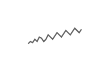
\begin{tikzpicture}[x=0.08em, y=0.08em, line width=0.4pt]
                \draw[FooterGray] (0,3) -- (1,4) -- (2,3.5) -- (3,5) -- (4,4) -- (5,6) -- (6,5.5) -- (7,4) -- (8,5) -- (9,7) -- (10,6) -- (11,5) -- (12,6.5) -- (13,8) -- (14,7) -- (15,6) -- (16,7.5) -- (17,9) -- (18,8) -- (19,7) -- (20,8.5) -- (21,10) -- (22,9) -- (23,8) -- (24,9.5);
            \end{tikzpicture}%
        }%
        \hskip0.5cm%
    }%
    \vskip6pt%
}

%=============================================================================
% PACKAGES
%=============================================================================
\usepackage[utf8]{inputenc}
\usepackage[T1]{fontenc}
\usepackage{amsmath, amssymb, amsthm}
\usepackage{mathtools}
\usepackage{bm}
\usepackage{tikz}
\usetikzlibrary{arrows.meta, positioning, shapes, calc, decorations.pathreplacing, shadings}
\usepackage{booktabs}
\usepackage{multirow}
\usepackage{array}
\usepackage{graphicx}
\usepackage{hyperref}
\usepackage{colortbl}
\usepackage{listings}
\lstset{language=Python, basicstyle=\ttfamily\scriptsize, keywordstyle=\color{MainBlue}\bfseries,
  commentstyle=\color{Forest}, stringstyle=\color{Crimson}, breaklines=true,
  frame=none, backgroundcolor=\color{VeryLightGray}, xleftmargin=2mm}
\hypersetup{colorlinks=true, linkcolor=MainBlue, urlcolor=MainBlue}
\graphicspath{{../../logos/}{../../charts/}{../../photos/}}
\hfuzz=2pt
\vfuzz=2pt

%=============================================================================
% QUANTLET COMMAND
%=============================================================================
\newcommand{\quantlet}[2]{%
    \hfill\href{#2}{%
        \raisebox{-0.15em}{
\includegraphics[height=0.7em]{ql_logo.png}}%
        \textcolor{MainBlue}{\tiny\ #1}%
    }%
}

%=============================================================================
% CUSTOM TITLE PAGE
%=============================================================================
\defbeamertemplate*{title page}{hybrid}[1][]
{
    \vspace{0.2cm}
    \begin{center}
        \href{https://www.ase.ro}{
\includegraphics[height=1.0cm]{ase_logo.png}}\hspace{0.3cm}%
        \href{https://theida.net}{
\includegraphics[height=1.0cm]{ida_logo.png}}\hspace{0.3cm}%
        \href{https://blockchain-research-center.com}{
\includegraphics[height=1.0cm]{brc_logo.png}}\hspace{0.3cm}%
        \href{https://www.ai4efin.ase.ro}{
\includegraphics[height=1.0cm]{ai4efin_logo.png}}\hspace{0.3cm}%
        \href{https://ipe.ro/new}{
\includegraphics[height=1.0cm]{acad_logo.png}}\hspace{0.3cm}%
        \href{https://www.digital-finance-msca.com}{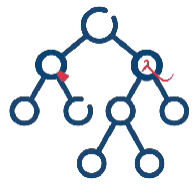
\includegraphics[height=1.0cm]{msca_logo.png}}%
    \end{center}

    \vspace{0.6cm}

    \begin{center}
        \begin{minipage}{0.1\textwidth}
            \centering
            \href{https://quantlet.com}{
\includegraphics[height=1.1cm]{ql_logo.png}}
        \end{minipage}%
        \begin{minipage}{0.78\textwidth}
            \centering
            {\LARGE\bfseries\usebeamercolor[fg]{title}\inserttitle}

            \vspace{0.3cm}

            {\usebeamerfont{subtitle}\usebeamercolor[fg]{title}\insertsubtitle}
        \end{minipage}%
        \begin{minipage}{0.1\textwidth}
            \centering
            \href{https://quantinar.com}{
\includegraphics[height=1.1cm]{qr_logo.png}}
        \end{minipage}
    \end{center}

    \vspace{0.6cm}

    \hspace{0.5cm}{\usebeamerfont{author}\insertauthor}

    \vspace{0.3cm}

    \hspace{0.5cm}\begin{minipage}[t]{0.9\textwidth}
        \raggedright\small\insertinstitute
    \end{minipage}
}

%=============================================================================
% THEOREM ENVIRONMENTS
%=============================================================================
\theoremstyle{definition}
\setbeamertemplate{theorems}[numbered]
\newtheorem{defn}{Definition}
\newtheorem{thm}{Theorem}
\newtheorem{prop}{Proposition}
\newtheorem{rmk}{Remark}

%=============================================================================
% CENTRED MINIPAGE
%=============================================================================
\newenvironment{cminipage}[1]{%
    \par\noindent\hfill\begin{minipage}{#1}\ignorespaces
}{%
    \end{minipage}\hfill\null\par
}

%=============================================================================
% CUSTOM COMMANDS
%=============================================================================
\newcommand{\E}{\mathbb{E}}
\newcommand{\Var}{\text{Var}}
\newcommand{\Cov}{\text{Cov}}
\newcommand{\Corr}{\text{Corr}}
\newcommand{\R}{\mathbb{R}}
\newcommand{\N}{\mathbb{N}}
\newcommand{\Z}{\mathbb{Z}}
\newcommand{\B}{\mathbf{B}}
\newcommand{\imark}{\textcolor{MainBlue}{\textbullet}}
\newcommand{\RMSE}{\text{RMSE}}
\newcommand{\MAE}{\text{MAE}}
\newcommand{\MAPE}{\text{MAPE}}

%=============================================================================
% TITLE INFORMATION
%=============================================================================
\title[Statistics of Financial Markets]{Statistics of Financial Markets}
\subtitle{Chapter 3: The Efficient Market Hypothesis}
\author[D.T. Pele]{Daniel Traian PELE}
\institute{Bucharest University of Economic Studies\\
IDA Institute Digital Assets\\
Blockchain Research Center\\
AI4EFin Artificial Intelligence for Energy Finance\\
Romanian Academy, Institute for Economic Forecasting\\
MSCA Digital Finance}
\date{}

%=============================================================================
\begin{document}
%=============================================================================

% Title page
{
\setbeamertemplate{headline}{}
\setbeamertemplate{footline}{}
\begin{frame}[plain]
    \titlepage
\end{frame}
}

%=============================================================================
% LEARNING OBJECTIVES
%=============================================================================
\begin{frame}{Learning Objectives}
    \begin{block}{By the end of this chapter, you will be able to:}
    \begin{enumerate}
        \item[\textcolor{MainBlue}{\textbf{1.}}] \textbf{Define} market efficiency and its three forms (weak, semi-strong, strong)
        \item[\textcolor{MainBlue}{\textbf{2.}}] \textbf{Formalize} the EMH using martingale and random walk models
        \item[\textcolor{MainBlue}{\textbf{3.}}] \textbf{Implement} statistical tests for weak-form efficiency (autocorrelation, runs, variance ratio)
        \item[\textcolor{MainBlue}{\textbf{4.}}] \textbf{Analyze} event studies for semi-strong efficiency
        \item[\textcolor{MainBlue}{\textbf{5.}}] \textbf{Evaluate} market anomalies and behavioral challenges to EMH
        \item[\textcolor{MainBlue}{\textbf{6.}}] \textbf{Discuss} the Adaptive Market Hypothesis as a modern synthesis
    \end{enumerate}
    \end{block}
\end{frame}

%=============================================================================
% TABLE OF CONTENTS
%=============================================================================
{
\setbeamertemplate{headline}{%
    \vskip10pt%
    \hbox to \paperwidth{\hskip0.5cm\hfill\hskip0.5cm}%
    \vskip4pt%
    {\color{FooterGray}\hrule height 0.4pt}%
}
\begin{frame}{}
    {\color{FooterGray}\hrule height 0.4pt}
    \vspace{0.1cm}
    {\Large\textcolor{IDAred}{\textbf{Contents}}}
    \vspace{0.2cm}
    {\small
    \begin{columns}[T]
        \begin{column}{0.48\textwidth}
            \begin{enumerate}
                \item Motivation
                \item The Efficient Market Hypothesis
                \item Mathematical Framework
                \item Weak-Form Efficiency
                \item Semi-Strong Efficiency
                \item Strong-Form Efficiency
            \end{enumerate}
        \end{column}
        \begin{column}{0.48\textwidth}
            \begin{enumerate}\setcounter{enumi}{6}
                \item Market Anomalies
                \item Behavioral Finance
                \item The Adaptive Market Hypothesis
                \item Case Studies
                \item Exercises and Python Labs
                \item Conclusions
            \end{enumerate}
        \end{column}
    \end{columns}
    }
\end{frame}
}

%#############################################################################
\section{Motivation}
%#############################################################################

\begin{frame}{Can You Beat the Market?}
\begin{cminipage}{0.95\textwidth}
\begin{columns}[T]
\begin{column}{0.55\textwidth}
\begin{itemize}\setlength{\itemsep}{0pt}
    \item \textbf{Central question in finance:} can an investor consistently earn returns above the market benchmark?
    \item Burton Malkiel (1973): ``A blindfolded monkey throwing darts at a newspaper's financial pages could select a portfolio that would do just as well as one carefully selected by experts.''
    \item \textbf{Empirical fact:} over 90\% of actively managed funds underperform their benchmark index over 15-year horizons (SPIVA Scorecard, 2024)
    \item If prices already reflect all available information, then no strategy can systematically generate \textbf{alpha}
\end{itemize}
\end{column}
\begin{column}{0.42\textwidth}
\begin{center}
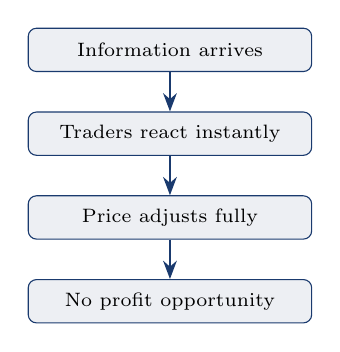
\begin{tikzpicture}[
    node distance=0.5cm,
    every node/.style={font=\scriptsize, align=center},
    phase/.style={draw=MainBlue, fill=MainBlue!8, rounded corners=3pt,
                  minimum width=3.6cm, minimum height=0.55cm}
]
\node[phase] (p1) {Information arrives};
\node[phase, below=of p1] (p2) {Traders react instantly};
\node[phase, below=of p2] (p3) {Price adjusts fully};
\node[phase, below=of p3] (p4) {No profit opportunity};
\draw[-{Stealth}, MainBlue, thick] (p1) -- (p2);
\draw[-{Stealth}, MainBlue, thick] (p2) -- (p3);
\draw[-{Stealth}, MainBlue, thick] (p3) -- (p4);
\end{tikzpicture}
\end{center}
\end{column}
\end{columns}
\end{cminipage}
\end{frame}

\begin{frame}{Historical Context}
\begin{cminipage}{0.95\textwidth}
\renewcommand{\arraystretch}{1.2}
\begin{center}
\begin{tabular}{lll}
\toprule
\textbf{Year} & \textbf{Author} & \textbf{Contribution} \\
\midrule
1900 & Louis Bachelier & Thesis: stock prices follow a random walk \\
1953 & Maurice Kendall & UK stock prices exhibit no predictable pattern \\
1965 & Eugene Fama & ``Random Walks in Stock Market Prices'' \\
1965 & Paul Samuelson & ``Proof That Properly Anticipated Prices Fluctuate Randomly'' \\
1970 & Eugene Fama & Formal EMH taxonomy: weak, semi-strong, strong \\
1991 & Eugene Fama & Revised EMH: return predictability, event studies, private info \\
2004 & Andrew Lo & Adaptive Market Hypothesis (AMH) \\
2013 & Fama \& Shiller & Nobel Prize (opposing views on efficiency) \\
\bottomrule
\end{tabular}
\end{center}
\end{cminipage}
\end{frame}

%#############################################################################
\section{The Efficient Market Hypothesis}
%#############################################################################

\begin{frame}{Definition of Market Efficiency}
\begin{cminipage}{0.95\textwidth}
\begin{defn}[Efficient Market --- Fama, 1970]
A market is \textbf{informationally efficient} if prices at any time $t$ fully reflect all available information $\Omega_t$. Formally:
$$P_t = \E[P_t \mid \Omega_t]$$
where $\Omega_t$ is the information set available at time $t$.
\end{defn}

\vspace{0.3cm}
\begin{itemize}\setlength{\itemsep}{0pt}
    \item \textbf{Implication:} no trading strategy based on $\Omega_t$ can yield expected returns exceeding the equilibrium return
    \item Price changes respond only to \textbf{new information} (surprises), which is by definition unpredictable
    \item The EMH is a \textbf{joint hypothesis}: efficiency + an equilibrium model of expected returns
\end{itemize}

\begin{alertblock}{Joint Hypothesis Problem}
\begin{itemize}\setlength{\itemsep}{0pt}
    \item We can never test efficiency alone --- any test requires an asset pricing model (CAPM, APT, etc.). A rejection might mean inefficiency \textit{or} a wrong model.
\end{itemize}
\end{alertblock}
\end{cminipage}
\end{frame}

\begin{frame}{Three Forms of the EMH}
\begin{cminipage}{0.95\textwidth}
\begin{center}
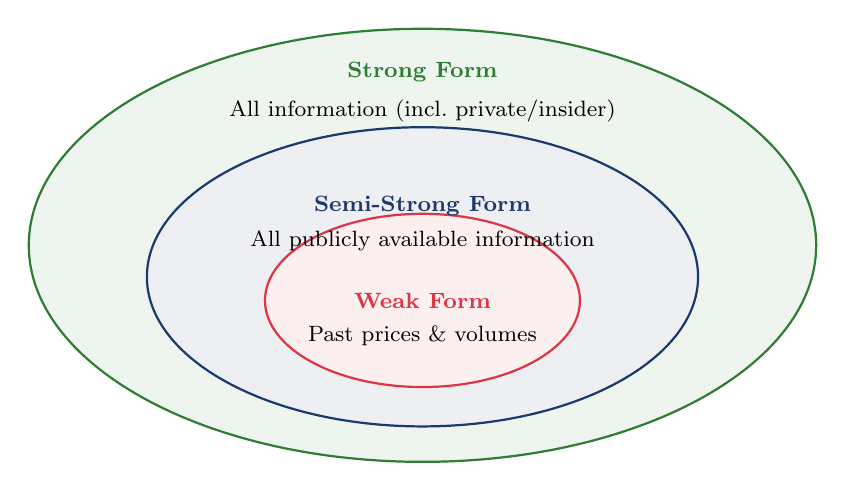
\begin{tikzpicture}[
    every node/.style={font=\small, align=center},
    circle1/.style={draw=Forest, fill=Forest!8, thick, ellipse, minimum width=10cm, minimum height=5.5cm},
    circle2/.style={draw=MainBlue, fill=MainBlue!8, thick, ellipse, minimum width=7cm, minimum height=3.8cm},
    circle3/.style={draw=Crimson, fill=Crimson!8, thick, ellipse, minimum width=4cm, minimum height=2.2cm}
]
\node[circle1] at (0,0) {};
\node[circle2] at (0,-0.4) {};
\node[circle3] at (0,-0.7) {};
\node[font=\footnotesize\bfseries, Forest] at (0, 2.2) {Strong Form};
\node[font=\footnotesize] at (0, 1.7) {All information (incl.\ private/insider)};
\node[font=\footnotesize\bfseries, MainBlue] at (0, 0.5) {Semi-Strong Form};
\node[font=\footnotesize] at (0, 0.05) {All publicly available information};
\node[font=\footnotesize\bfseries, Crimson] at (0, -0.7) {Weak Form};
\node[font=\footnotesize] at (0, -1.15) {Past prices \& volumes};
\end{tikzpicture}
\end{center}
\end{cminipage}
\end{frame}

\begin{frame}{The Three Forms: Summary}
\begin{cminipage}{0.95\textwidth}
\small
\renewcommand{\arraystretch}{1.2}
\begin{center}
\scriptsize
\renewcommand{\arraystretch}{1.3}
\begin{tabular}{llll}
\toprule
\textbf{Form} & \textbf{Information set} & \textbf{Implication} & \textbf{What it rules out} \\
\midrule
\textbf{Weak} & Past prices, volumes & Tech.\ analysis $\not\Rightarrow$ $\alpha$ & Moving averages, chart patterns \\
\textbf{Semi-strong} & All public info & Fund.\ analysis $\not\Rightarrow$ $\alpha$ & Earnings strategies, news trading \\
\textbf{Strong} & All info (incl.\ insider) & No investor has edge & Insider trading, private tips \\
\bottomrule
\end{tabular}
\end{center}

\vspace{0.3cm}
\begin{itemize}\setlength{\itemsep}{0pt}
    \item Each form is \textbf{nested}: strong $\Rightarrow$ semi-strong $\Rightarrow$ weak
    \item If the strong form holds, both weaker forms hold automatically
    \item Most empirical research focuses on weak and semi-strong efficiency
\end{itemize}
\end{cminipage}
\end{frame}

%#############################################################################
\section{Mathematical Framework}
%#############################################################################

\begin{frame}{Fair Game Model}
\begin{cminipage}{0.95\textwidth}
\begin{defn}[Fair Game]
Let $r_{t+1}$ be the return on an asset. The market is a \textbf{fair game} with respect to information $\Omega_t$ if:
$$\E[r_{t+1} - \E[r_{t+1} \mid \Omega_t] \mid \Omega_t] = 0$$
\end{defn}

\begin{itemize}\setlength{\itemsep}{0pt}
    \item Define excess return: $z_{t+1} = r_{t+1} - \E[r_{t+1} \mid \Omega_t]$
    \item Fair game condition: $\E[z_{t+1} \mid \Omega_t] = 0$ --- forecast errors are unbiased
    \item No trading rule $\delta(\Omega_t)$ can produce positive expected excess profit:
    $$\E[\delta(\Omega_t) \cdot z_{t+1}] = 0$$
\end{itemize}

\begin{exampleblock}{Intuition}
\begin{itemize}\setlength{\itemsep}{0pt}
    \item A fair game does not mean returns are zero --- it means \textbf{unexpected} returns are zero on average. Investors earn the equilibrium risk premium, but cannot consistently do better.
\end{itemize}
\end{exampleblock}
\end{cminipage}
\end{frame}

\begin{frame}{Martingale and Random Walk}
\begin{cminipage}{0.95\textwidth}
\begin{columns}[T]
\begin{column}{0.48\textwidth}
\begin{block}{Martingale}
\begin{itemize}\setlength{\itemsep}{0pt}
    \item $\{P_t\}$ is a martingale w.r.t.\ $\Omega_t$ if:
    $$\E[P_{t+1} \mid \Omega_t] = P_t$$
    \item Prices have no predictable drift
    \item Weaker than random walk: allows for time-varying variance
\end{itemize}
\end{block}
\end{column}
\begin{column}{0.48\textwidth}
\begin{block}{Random Walk}
\begin{itemize}\setlength{\itemsep}{0pt}
    \item \textbf{RW1:} $P_t = P_{t-1} + \varepsilon_t$, $\varepsilon_t \stackrel{iid}{\sim}(0, \sigma^2)$
    \item \textbf{RW2:} increments are independent but not identically distributed
    \item \textbf{RW3:} increments are uncorrelated (weakest)
    \item RW1 $\Rightarrow$ RW2 $\Rightarrow$ RW3
\end{itemize}
\end{block}
\end{column}
\end{columns}

\vspace{0.3cm}
\begin{alertblock}{Key Distinction}
\begin{itemize}\setlength{\itemsep}{0pt}
    \item EMH $\not\Leftrightarrow$ Random Walk. EMH implies a \textbf{martingale} for risk-adjusted prices, not necessarily iid increments. Volatility clustering is compatible with EMH.
\end{itemize}
\end{alertblock}
\end{cminipage}
\end{frame}

\begin{frame}{From EMH to Testable Predictions}
\begin{cminipage}{0.95\textwidth}
\begin{center}
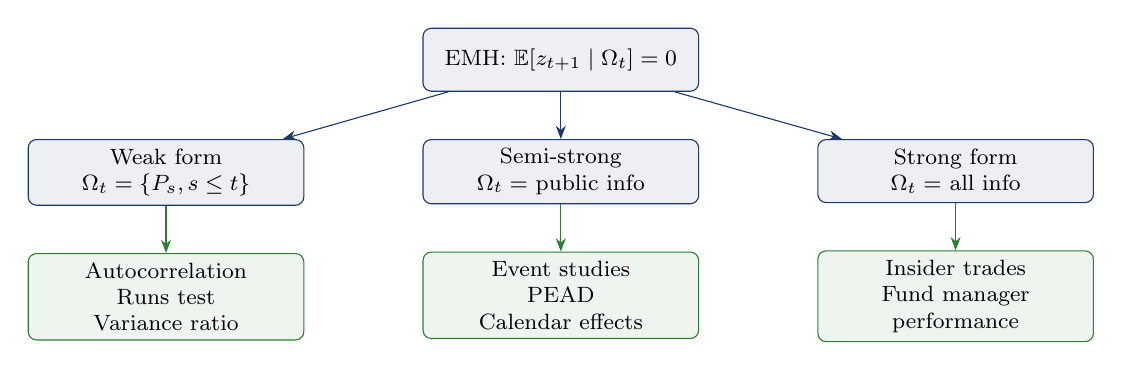
\begin{tikzpicture}[
    node distance=0.6cm and 1.5cm,
    every node/.style={font=\small, align=center},
    box/.style={draw=MainBlue, fill=MainBlue!8, rounded corners=3pt,
                minimum width=3.5cm, minimum height=0.8cm, font=\footnotesize},
    test/.style={draw=Forest, fill=Forest!8, rounded corners=3pt,
                minimum width=3.5cm, minimum height=0.8cm, font=\footnotesize}
]
\node[box] (emh) {EMH: $\E[z_{t+1}\mid\Omega_t]=0$};
\node[box, below left=of emh] (weak) {Weak form\\$\Omega_t = \{P_s, s \leq t\}$};
\node[box, below=of emh] (semi) {Semi-strong\\$\Omega_t =$ public info};
\node[box, below right=of emh] (strong) {Strong form\\$\Omega_t =$ all info};

\node[test, below=of weak] (t1) {Autocorrelation\\Runs test\\Variance ratio};
\node[test, below=of semi] (t2) {Event studies\\PEAD\\Calendar effects};
\node[test, below=of strong] (t3) {Insider trades\\Fund manager\\performance};

\draw[-{Stealth}, MainBlue] (emh) -- (weak);
\draw[-{Stealth}, MainBlue] (emh) -- (semi);
\draw[-{Stealth}, MainBlue] (emh) -- (strong);
\draw[-{Stealth}, Forest] (weak) -- (t1);
\draw[-{Stealth}, Forest] (semi) -- (t2);
\draw[-{Stealth}, Forest] (strong) -- (t3);
\end{tikzpicture}
\end{center}
\end{cminipage}
\end{frame}

%#############################################################################
\section{Weak-Form Efficiency}
%#############################################################################

\begin{frame}{Testing Weak-Form Efficiency}
\begin{cminipage}{0.95\textwidth}
\begin{itemize}\setlength{\itemsep}{0pt}
    \item \textbf{Null hypothesis:} past returns contain no information about future returns
    \item If weak-form EMH holds, returns should be serially uncorrelated:
$$\Corr(r_t, r_{t-k}) = 0, \quad \forall\, k \geq 1$$
\end{itemize}

\vspace{0.2cm}
\begin{block}{Main Statistical Tests}
\renewcommand{\arraystretch}{1.2}
\small
\begin{tabular}{lll}
\toprule
\textbf{Test} & \textbf{Null hypothesis} & \textbf{Method} \\
\midrule
Autocorrelation & $\rho_k = 0$ for all $k$ & Ljung--Box $Q$-statistic \\
Runs test & Returns are random & Non-parametric sign test \\
Variance ratio & $\Var(r_t^{(q)}) = q \cdot \Var(r_t)$ & Lo--MacKinlay (1988) \\
ADF test & Unit root in prices & Augmented Dickey--Fuller \\
\bottomrule
\end{tabular}
\end{block}
\end{cminipage}
\end{frame}

\begin{frame}{Autocorrelation Test}
\begin{cminipage}{0.95\textwidth}
\begin{columns}[T]
\begin{column}{0.48\textwidth}
\begin{block}{Sample Autocorrelation}
$$\hat{\rho}_k = \frac{\sum_{t=k+1}^{T}(r_t - \bar{r})(r_{t-k} - \bar{r})}{\sum_{t=1}^{T}(r_t - \bar{r})^2}$$
\end{block}

\begin{itemize}\setlength{\itemsep}{0pt}
    \item Under $H_0$: $\hat{\rho}_k \sim \mathcal{N}(0, 1/T)$ approximately
    \item Reject if $|\hat{\rho}_k| > z_{\alpha/2}/\sqrt{T}$
\end{itemize}
\end{column}
\begin{column}{0.48\textwidth}
\begin{block}{Ljung--Box $Q$-Statistic}
$$Q(m) = T(T+2)\sum_{k=1}^{m}\frac{\hat{\rho}_k^2}{T-k}$$
\end{block}

\begin{itemize}\setlength{\itemsep}{0pt}
    \item Tests joint null: $\rho_1 = \rho_2 = \cdots = \rho_m = 0$
    \item Under $H_0$: $Q(m) \sim \chi^2(m)$
    \item Typical choice: $m = 10$ or $m = 20$
\end{itemize}
\end{column}
\end{columns}

\vspace{0.2cm}
\begin{exampleblock}{Empirical Finding}
\begin{itemize}\setlength{\itemsep}{0pt}
    \item Daily returns on major indices show small but statistically significant $\hat{\rho}_1 \approx 0.05$--$0.10$ (Lo \& MacKinlay, 1988). Economically small, but challenges strict weak-form EMH.
\end{itemize}
\end{exampleblock}
\end{cminipage}
\quantlet{SFM\_ch3\_emh\_tests}{https://github.com/QuantLet/Stat_fin_markets/tree/master/Ch_03/SFM_ch3_emh_tests}
\end{frame}

%--- Code Slide: Autocorrelation + Ljung-Box ---
\begin{frame}[fragile]{Python: Autocorrelation and Ljung--Box Test}
\begin{cminipage}{0.95\textwidth}
\begin{lstlisting}
import yfinance as yf
import numpy as np
from statsmodels.stats.diagnostic import acorr_ljungbox
from statsmodels.tsa.stattools import acf

# Download S&P 500 data and compute log-returns
sp = yf.download('^GSPC', start='2015-01-01', end='2025-01-01')
prices = sp['Adj Close'].dropna()
returns = np.log(prices / prices.shift(1)).dropna()

# Sample autocorrelations (first 20 lags)
acf_vals = acf(returns, nlags=20, fft=True)
print("ACF lags 1-5:", np.round(acf_vals[1:6], 4))

# Ljung-Box test (H0: no autocorrelation up to lag m)
lb = acorr_ljungbox(returns, lags=[10, 20], return_df=True)
print(lb)  # If p-value < 0.05, reject weak-form EMH
\end{lstlisting}
\end{cminipage}
\quantlet{SFM\_ch3\_emh\_tests}{https://github.com/QuantLet/Stat_fin_markets/tree/master/Ch_03/SFM_ch3_emh_tests}
\end{frame}

%--- ACF Plot Description ---
\begin{frame}{Autocorrelation Function of S\&P 500 Returns}
\begin{cminipage}{0.95\textwidth}
\begin{columns}[T]
\begin{column}{0.48\textwidth}
\begin{block}{ACF of Returns $r_t$}
\begin{itemize}\setlength{\itemsep}{0pt}
    \item Autocorrelations are very small: $|\hat{\rho}_k| < 0.05$ for most lags
    \item A few lags may be marginally significant (barely outside $\pm 1.96/\sqrt{T}$ bands)
    \item \textbf{Consistent with weak-form EMH}: returns are approximately unpredictable
\end{itemize}
\end{block}
\end{column}
\begin{column}{0.48\textwidth}
\begin{block}{ACF of $|r_t|$ and $r_t^2$}
\begin{itemize}\setlength{\itemsep}{0pt}
    \item Absolute and squared returns show \textbf{strong, persistent} autocorrelation
    \item $\hat{\rho}_k(|r_t|) > 0$ for $k = 1, \ldots, 100+$
    \item This is \textbf{volatility clustering}: compatible with EMH (martingale allows time-varying variance)
    \item Key distinction: \textbf{returns} are unpredictable, but \textbf{volatility} is predictable
\end{itemize}
\end{block}
\end{column}
\end{columns}

\vspace{0.2cm}
\begin{alertblock}{Important}
\begin{itemize}\setlength{\itemsep}{0pt}
    \item Predictable volatility $\neq$ predictable returns. EMH is about the \textbf{direction} of price changes, not their magnitude.
\end{itemize}
\end{alertblock}
\end{cminipage}
\quantlet{SFM\_ch3\_emh\_tests}{https://github.com/QuantLet/Stat_fin_markets/tree/master/Ch_03/SFM_ch3_emh_tests}
\end{frame}

\begin{frame}{Autocorrelation Function: Empirical Results}
\begin{cminipage}{0.95\textwidth}
\begin{center}
\IfFileExists{ch3_emh_tests.pdf}{%
    
\includegraphics[width=0.55\textwidth]{ch3_emh_tests.pdf}
}{%
    \textit{[Chart: ACF of S\&P 500 returns and squared returns --- ch3\_emh\_tests.pdf]}
}
\end{center}
\begin{itemize}\setlength{\itemsep}{0pt}
    \item \textbf{Left:} ACF of returns --- all bars within the 95\% confidence band
    \item \textbf{Right:} ACF of $r_t^2$ --- significant persistent autocorrelation (volatility clustering)
\end{itemize}
\end{cminipage}
\quantlet{SFM\_ch3\_emh\_tests}{https://github.com/QuantLet/Stat_fin_markets/tree/master/Ch_03/SFM_ch3_emh_tests}
\end{frame}

\begin{frame}{The Runs Test}
\begin{cminipage}{0.95\textwidth}
\begin{defn}[Run]
A \textbf{run} is a maximal consecutive sequence of returns with the same sign. E.g., $(+,+,-,-,-,+)$ has 3 runs.
\end{defn}

\begin{columns}[T]
\begin{column}{0.48\textwidth}
\begin{itemize}\setlength{\itemsep}{0pt}
    \item Let $n_+$ = number of positive returns, $n_-$ = number of negative returns, $R$ = number of runs
    \item Under independence:
    $$\E[R] = \frac{2n_+n_-}{n_+ + n_-} + 1$$
    $$\Var(R) = \frac{2n_+n_-(2n_+n_- - n_+ - n_-)}{(n_++n_-)^2(n_++n_--1)}$$
\end{itemize}
\end{column}
\begin{column}{0.48\textwidth}
\begin{itemize}\setlength{\itemsep}{0pt}
    \item Test statistic:
    $$Z = \frac{R - \E[R]}{\sqrt{\Var(R)}} \xrightarrow{d} \mathcal{N}(0,1)$$
    \item \textbf{Too few runs} $\Rightarrow$ momentum (positive autocorrelation)
    \item \textbf{Too many runs} $\Rightarrow$ mean reversion (negative autocorrelation)
    \item Non-parametric: no distributional assumption needed
\end{itemize}
\end{column}
\end{columns}
\end{cminipage}
\quantlet{SFM\_ch3\_emh\_tests}{https://github.com/QuantLet/Stat_fin_markets/tree/master/Ch_03/SFM_ch3_emh_tests}
\end{frame}

\begin{frame}{The Variance Ratio Test}
\begin{cminipage}{0.95\textwidth}
\begin{block}{Key Idea}
\begin{itemize}\setlength{\itemsep}{0pt}
    \item If returns are iid, the variance of $q$-period returns should scale linearly: $\Var(r_t(q)) = q \cdot \Var(r_t)$
\end{itemize}
\end{block}

\begin{columns}[T]
\begin{column}{0.50\textwidth}
\begin{itemize}\setlength{\itemsep}{0pt}
    \item \textbf{Variance ratio:}
    $$VR(q) = \frac{\Var(r_t(q))}{q \cdot \Var(r_t)} = 1 + 2\sum_{k=1}^{q-1}\left(1 - \frac{k}{q}\right)\rho_k$$
    \item $VR(q) = 1$: random walk (no autocorrelation)
    \item $VR(q) > 1$: positive autocorrelation (momentum)
    \item $VR(q) < 1$: negative autocorrelation (mean reversion)
\end{itemize}
\end{column}
\begin{column}{0.46\textwidth}
\begin{itemize}\setlength{\itemsep}{0pt}
    \item \textbf{Lo--MacKinlay (1988):}
    $$Z(q) = \frac{VR(q) - 1}{\sqrt{\phi(q)}} \xrightarrow{d} \mathcal{N}(0,1)$$
    where $\phi(q)$ is the asymptotic variance
    \item Heteroscedasticity-robust version available
    \item Typical: $q = 2, 5, 10, 20$
\end{itemize}

\end{column}
\end{columns}
\end{cminipage}
\quantlet{SFM\_ch3\_variance\_ratio}{https://github.com/QuantLet/Stat_fin_markets/tree/master/Ch_03/SFM_ch3_variance_ratio}
\end{frame}

%--- Code Slide: Variance Ratio Test ---
\begin{frame}[fragile]{Python: Variance Ratio Test on S\&P 500}
\begin{cminipage}{0.95\textwidth}
\begin{lstlisting}
import numpy as np
import yfinance as yf

sp = yf.download('^GSPC', start='2015-01-01', end='2025-01-01')
r = np.log(sp['Adj Close'] / sp['Adj Close'].shift(1)).dropna().values

def variance_ratio(returns, q):
    """Lo-MacKinlay variance ratio test."""
    T = len(returns)
    mu = returns.mean()
    # Variance of 1-period returns
    sig1 = np.sum((returns - mu)**2) / (T - 1)
    # q-period returns
    rq = np.array([returns[i:i+q].sum() for i in range(T - q + 1)])
    sigq = np.sum((rq - q * mu)**2) / (T - 1)
    VR = sigq / (q * sig1)
    # Asymptotic z-statistic (homoscedastic)
    phi = 2 * (2*q - 1) * (q - 1) / (3 * q * T)
    z = (VR - 1) / np.sqrt(phi)
    return VR, z

for q in [2, 5, 10, 20]:
    vr, z = variance_ratio(r, q)
    print(f"VR({q:2d}) = {vr:.4f},  z = {z:+.3f}")
\end{lstlisting}
\end{cminipage}
\quantlet{SFM\_ch3\_variance\_ratio}{https://github.com/QuantLet/Stat_fin_markets/tree/master/Ch_03/SFM_ch3_variance_ratio}
\end{frame}

\begin{frame}{Variance Ratio: Empirical Results}
\begin{cminipage}{0.95\textwidth}
\small
\renewcommand{\arraystretch}{1.2}
\begin{center}
\begin{tabular}{lccccl}
\toprule
\textbf{Market} & $VR(2)$ & $VR(5)$ & $VR(10)$ & $VR(20)$ & \textbf{Interpretation} \\
\midrule
S\&P 500 (daily) & 1.05 & 1.04 & 0.99 & 0.95 & Short-term momentum, long-term reversion \\
FTSE 100 (daily) & 1.03 & 1.01 & 0.97 & 0.92 & Mild mean reversion \\
BTC-USD (daily) & 1.02 & 0.98 & 0.94 & 0.88 & Mean reversion at longer horizons \\
BET (daily) & 1.12 & 1.18 & 1.10 & 1.01 & Stronger momentum (less efficient) \\
\bottomrule
\end{tabular}
\end{center}

\vspace{0.2cm}
\begin{itemize}\setlength{\itemsep}{0pt}
    \item Developed markets: $VR \approx 1$ at most horizons $\Rightarrow$ approximately efficient
    \item Emerging markets (BET): larger deviations $\Rightarrow$ potential inefficiency
    \item Crypto: high short-term efficiency, long-term mean reversion
    \item \textbf{Pattern:} VR $> 1$ at short horizons, VR $< 1$ at long horizons --- consistent with short-term momentum and long-term mean reversion (Poterba \& Summers, 1988)
\end{itemize}
\end{cminipage}
\end{frame}

\begin{frame}{Variance Ratio: Graphical Comparison}
\begin{cminipage}{0.95\textwidth}
\begin{center}
\IfFileExists{ch3_variance_ratio.pdf}{%
    
\includegraphics[width=0.55\textwidth]{ch3_variance_ratio.pdf}
}{%
    \textit{[Chart: Variance ratio $VR(q)$ for S\&P 500, BET, BTC-USD --- ch3\_variance\_ratio.pdf]}
}
\end{center}
\begin{itemize}\setlength{\itemsep}{0pt}
    \item $VR(q)$ for $q = 2, 5, 10, 20$ with 95\% confidence bands
    \item Developed markets: $VR \approx 1$; emerging markets: significant deviations
\end{itemize}
\end{cminipage}
\quantlet{SFM\_ch3\_variance\_ratio}{https://github.com/QuantLet/Stat_fin_markets/tree/master/Ch_03/SFM_ch3_variance_ratio}
\end{frame}

%--- Random Walk Types ---
\begin{frame}{Random Walk Types: Formal Definitions}
\begin{cminipage}{0.95\textwidth}
\footnotesize
\begin{defn}[Random Walk 1 --- IID increments]
$P_t = \mu + P_{t-1} + \varepsilon_t$, \; $\varepsilon_t \stackrel{iid}{\sim} F(0, \sigma^2)$. \;
Strongest form: increments are independent and identically distributed.
\end{defn}
\vspace{-1mm}
\begin{defn}[Random Walk 2 --- Independent increments]
$P_t = \mu + P_{t-1} + \varepsilon_t$, \; $\varepsilon_t$ independent but $\varepsilon_t \sim F_t(0, \sigma_t^2)$. \;
Allows heteroscedasticity (time-varying variance). Compatible with GARCH.
\end{defn}
\vspace{-1mm}
\begin{defn}[Random Walk 3 --- Uncorrelated increments]
$P_t = \mu + P_{t-1} + \varepsilon_t$, \; $\Cov(\varepsilon_t, \varepsilon_s) = 0$ for $t \neq s$. \;
Weakest: only zero autocorrelation. Allows dependence in higher moments.
\end{defn}
\vspace{-1mm}
\begin{alertblock}{Test Mapping}
\begin{itemize}\setlength{\itemsep}{0pt}
    \item Autocorrelation/LB $\to$ RW3; \; VR (homoscedastic) $\to$ RW1; \; VR (robust) $\to$ RW2; \; Runs/BDS $\to$ RW2
\end{itemize}
\end{alertblock}
\end{cminipage}
\end{frame}

%--- Logarithmic Random Walk ---
\begin{frame}[shrink=5]{Logarithmic Random Walk}
\begin{cminipage}{0.95\textwidth}
\begin{block}{The Model}
\begin{itemize}\setlength{\itemsep}{0pt}
    \item Financial prices follow a \textbf{geometric random walk}:
    $$P_t = P_{t-1} \cdot e^{\mu + \sigma\varepsilon_t}, \quad \varepsilon_t \sim \mathcal{N}(0,1)$$
    \item Equivalently, log-prices follow an arithmetic random walk:
    $$\ln P_t = \ln P_{t-1} + \mu + \sigma\varepsilon_t$$
    \item Log-returns are i.i.d.:
    $$r_t = \ln\frac{P_t}{P_{t-1}} = \mu + \sigma\varepsilon_t \stackrel{iid}{\sim} \mathcal{N}(\mu, \sigma^2)$$
\end{itemize}
\end{block}

\begin{columns}[T]
\begin{column}{0.48\textwidth}
\begin{itemize}\setlength{\itemsep}{0pt}
    \item \textbf{Why logarithmic?}
    \item Prices cannot be negative: $P_t > 0$ always
    \item Log-returns are additively composable
    \item Consistent with continuous compounding
    \item Log-normality implies heavier tails than the simple normal
\end{itemize}
\end{column}
\begin{column}{0.48\textwidth}
\begin{itemize}\setlength{\itemsep}{0pt}
    \item \textbf{Properties:}
    \item $\E[\ln P_t] = \ln P_0 + \mu t$
    \item $\Var(\ln P_t) = \sigma^2 t$ (grows linearly)
    \item $P_t \sim \text{LogNormal}(\ln P_0 + \mu t, \sigma^2 t)$
    \item Square-root-of-time rule: $\sigma_{T\text{ days}} = \sigma_{1\text{ day}} \cdot \sqrt{T}$
\end{itemize}
\end{column}
\end{columns}
\end{cminipage}
\end{frame}

%--- Unit Root Tests ---
\begin{frame}{Unit Root Tests: ADF and Phillips--Perron}
\begin{cminipage}{0.95\textwidth}
\small
\begin{block}{Augmented Dickey--Fuller (ADF) Test}
\begin{itemize}\setlength{\itemsep}{0pt}
    \item Test regression: $\Delta P_t = \alpha + \gamma P_{t-1} + \sum_{j=1}^{p} \delta_j \Delta P_{t-j} + \varepsilon_t$
    \item $H_0$: $\gamma = 0$ (unit root $\Rightarrow$ random walk); \; $H_1$: $\gamma < 0$ (stationary)
    \item Test statistic: $\tau = \hat{\gamma} / \text{SE}(\hat{\gamma})$; Dickey--Fuller critical values (non-standard)
\end{itemize}
\end{block}

\begin{columns}[T]
\begin{column}{0.48\textwidth}
\begin{exampleblock}{Typical Results}
\begin{itemize}\setlength{\itemsep}{0pt}
    \item \textbf{Prices}: fail to reject $H_0$ $\Rightarrow$ unit root
    \item \textbf{Returns}: reject $H_0$ strongly $\Rightarrow$ stationary
    \item Confirms working with log-returns
\end{itemize}
\end{exampleblock}
\end{column}
\begin{column}{0.48\textwidth}
\begin{alertblock}{Phillips--Perron Test}
\begin{itemize}\setlength{\itemsep}{0pt}
    \item Non-parametric correction for serial correlation
    \item No lag selection needed
    \item More robust with heteroscedastic errors
\end{itemize}
\end{alertblock}
\end{column}
\end{columns}
\end{cminipage}
\quantlet{SFM\_ch3\_emh\_tests}{https://github.com/QuantLet/Stat_fin_markets/tree/master/Ch_03/SFM_ch3_emh_tests}
\end{frame}

%--- Spectral Analysis ---
\begin{frame}{Spectral Analysis for Testing Weak-Form EMH}
\begin{cminipage}{0.95\textwidth}
\begin{block}{Idea}
\begin{itemize}\setlength{\itemsep}{0pt}
    \item A random walk has a \textbf{flat spectrum} (white noise): equal power at all frequencies
    \item Peaks in the spectral density indicate predictable periodic components
\end{itemize}
\end{block}

\begin{columns}[T]
\begin{column}{0.48\textwidth}
\begin{itemize}\setlength{\itemsep}{0pt}
    \item \textbf{Spectral density} of a stationary process:
    $$f(\omega) = \frac{1}{2\pi}\sum_{k=-\infty}^{\infty}\gamma_k e^{-ik\omega}, \quad \omega \in [-\pi, \pi]$$
    where $\gamma_k = \Cov(r_t, r_{t-k})$
    \item Under RW3: $f(\omega) = \sigma^2/(2\pi)$ (constant)
    \item Estimated via periodogram or smoothed periodogram
\end{itemize}
\end{column}
\begin{column}{0.48\textwidth}
\begin{itemize}\setlength{\itemsep}{0pt}
    \item \textbf{Bartlett test}: tests flatness of the spectrum
    \item \textbf{Fisher test}: detects dominant periodicities
    \item Empirical findings for daily stock returns:
    \begin{itemize}\setlength{\itemsep}{0pt}
        \item Spectrum is approximately flat $\Rightarrow$ weak-form efficiency
        \item Small peaks at weekly/monthly frequencies in some markets
        \item Intraday data may show periodic patterns (market microstructure)
    \end{itemize}
\end{itemize}
\end{column}
\end{columns}
\end{cminipage}
\end{frame}

%--- Rolling Variance Ratio ---
\begin{frame}{Rolling Variance Ratio: Time-Varying Efficiency}
\begin{cminipage}{0.95\textwidth}
\small
\begin{block}{Methodology}
\begin{itemize}\setlength{\itemsep}{0pt}
    \item Compute $VR(q)$ over a rolling window of $W = 500$ days; plot $|VR(q) - 1|$ as efficiency index
\end{itemize}
\end{block}

\vspace{0.1cm}
\scriptsize
\renewcommand{\arraystretch}{1.1}
\begin{center}
\begin{tabular}{llll}
\toprule
\textbf{Period} & \textbf{S\&P 500 $|VR(5)-1|$} & \textbf{BET $|VR(5)-1|$} & \textbf{Interpretation} \\
\midrule
2005--2007 (calm) & 0.02 & 0.15 & SP efficient, BET less so \\
2008--2009 (GFC) & 0.12 & 0.25 & Both less efficient in crisis \\
2010--2019 (recovery) & 0.03 & 0.10 & Efficiency restored \\
2020 (Covid) & 0.08 & 0.18 & Temporary inefficiency spike \\
2021--2024 (post) & 0.03 & 0.08 & Back to normal \\
\bottomrule
\end{tabular}
\end{center}

\small
\begin{alertblock}{Key Finding}
\begin{itemize}\setlength{\itemsep}{0pt}
    \item Market efficiency is \textbf{not constant} --- it varies with market conditions. This supports the AMH over static EMH.
\end{itemize}
\end{alertblock}
\end{cminipage}
\quantlet{SFM\_ch3\_variance\_ratio}{https://github.com/QuantLet/Stat_fin_markets/tree/master/Ch_03/SFM_ch3_variance_ratio}
\end{frame}

%--- ADF Formal Setup ---
\begin{frame}{ADF Test: Formal Setup}
\begin{cminipage}{0.95\textwidth}
\small
\begin{block}{ADF Regression Equation}
\begin{itemize}\setlength{\itemsep}{0pt}
    \item Three variants depending on deterministic terms:
    \item \textbf{(i)} $\Delta y_t = \gamma y_{t-1} + \sum_{j=1}^{p}\delta_j \Delta y_{t-j} + \varepsilon_t$ \hfill (no constant, no trend)
    \item \textbf{(ii)} $\Delta y_t = \alpha + \gamma y_{t-1} + \sum_{j=1}^{p}\delta_j \Delta y_{t-j} + \varepsilon_t$ \hfill (constant, no trend)
    \item \textbf{(iii)} $\Delta y_t = \alpha + \beta t + \gamma y_{t-1} + \sum_{j=1}^{p}\delta_j \Delta y_{t-j} + \varepsilon_t$ \hfill (constant + trend)
\end{itemize}
\end{block}

\vspace{0.1cm}
\begin{columns}[T]
\begin{column}{0.48\textwidth}
\begin{itemize}\setlength{\itemsep}{0pt}
    \item \textbf{Lag selection:} choose $p$ via AIC or BIC
    \item AIC: $\ln(\hat{\sigma}^2) + 2p/T$
    \item BIC: $\ln(\hat{\sigma}^2) + p\ln(T)/T$
    \item BIC penalizes more $\Rightarrow$ selects fewer lags
\end{itemize}
\end{column}
\begin{column}{0.48\textwidth}
\footnotesize
\renewcommand{\arraystretch}{1.1}
\begin{tabular}{lll}
\toprule
\textbf{Signif.} & \textbf{No trend} & \textbf{With trend} \\
\midrule
1\% & $-3.43$ & $-3.96$ \\
5\% & $-2.86$ & $-3.41$ \\
10\% & $-2.57$ & $-3.13$ \\
\bottomrule
\end{tabular}
\begin{itemize}\setlength{\itemsep}{0pt}
    \item MacKinnon (1996) critical values
    \item Non-standard distribution
\end{itemize}
\end{column}
\end{columns}
\end{cminipage}
\end{frame}

%--- PP and KPSS ---
\begin{frame}{Phillips--Perron and KPSS Tests}
\begin{cminipage}{0.95\textwidth}
\small
\begin{columns}[T]
\begin{column}{0.48\textwidth}
\begin{block}{Phillips--Perron (PP) Test}
\begin{itemize}\setlength{\itemsep}{0pt}
    \item Regression: $\Delta y_t = \alpha + \gamma y_{t-1} + \varepsilon_t$
    \item Non-parametric Newey--West correction for serial correlation in $\varepsilon_t$
    \item No lag augmentation needed
    \item $H_0$: unit root ($\gamma = 0$)
    \item More robust under heteroscedasticity
\end{itemize}
\end{block}
\end{column}
\begin{column}{0.48\textwidth}
\begin{alertblock}{KPSS Test}
\begin{itemize}\setlength{\itemsep}{0pt}
    \item \textbf{Reverses the null}: $H_0$: stationarity
    \item Decomposition: $y_t = \xi t + r_t + \varepsilon_t$ where $r_t$ is a random walk
    \item Tests $\Var(r_t) = 0$ via LM statistic
    \item Rejects $\Rightarrow$ series has a unit root
\end{itemize}
\end{alertblock}
\end{column}
\end{columns}

\vspace{0.2cm}
\footnotesize
\renewcommand{\arraystretch}{1.1}
\begin{center}
\begin{tabular}{llll}
\toprule
\textbf{Feature} & \textbf{ADF} & \textbf{PP} & \textbf{KPSS} \\
\midrule
$H_0$ & Unit root & Unit root & Stationarity \\
Serial corr.\ fix & Lag augmentation & Newey--West & Bandwidth \\
Trend option & Yes & Yes & Yes \\
Power & Low for near-unit-root & Similar to ADF & Better size \\
\bottomrule
\end{tabular}
\end{center}
\end{cminipage}
\end{frame}

%--- Filter Rules ---
\begin{frame}{Filter Rules and Technical Trading}
\begin{cminipage}{0.95\textwidth}
\small
\begin{block}{Alexander Filter Rules}
\begin{itemize}\setlength{\itemsep}{0pt}
    \item Buy when price rises $x\%$ from a recent trough; sell when it falls $x\%$ from a recent peak
    \item If the market is weak-form efficient, no filter rule should outperform buy-and-hold after costs
\end{itemize}
\end{block}

\vspace{0.1cm}
\begin{columns}[T]
\begin{column}{0.48\textwidth}
\footnotesize
\renewcommand{\arraystretch}{1.1}
\begin{tabular}{lll}
\toprule
\textbf{Filter} & \textbf{Return} & \textbf{After costs} \\
\midrule
$x = 0.5\%$ & $+2.1\%$ & $-5.3\%$ \\
$x = 1\%$ & $+1.8\%$ & $-2.6\%$ \\
$x = 2\%$ & $+0.9\%$ & $-1.1\%$ \\
$x = 5\%$ & $-0.2\%$ & $-1.9\%$ \\
Buy-and-hold & $+8.2\%$ & $+8.0\%$ \\
\bottomrule
\end{tabular}
\end{column}
\begin{column}{0.48\textwidth}
\begin{itemize}\setlength{\itemsep}{0pt}
    \item \textbf{MA crossover:} buy when short MA crosses above long MA
    \item Popular: MA(50) vs MA(200) (``golden cross'' / ``death cross'')
    \item Fama \& Blume (1966): filters profitable before costs, not after
    \item Most technical rules fail after realistic transaction costs
\end{itemize}
\end{column}
\end{columns}

\vspace{0.1cm}
\begin{exampleblock}{Implication}
\begin{itemize}\setlength{\itemsep}{0pt}
    \item Filter rule results are consistent with weak-form EMH: any small predictability is consumed by costs
\end{itemize}
\end{exampleblock}
\end{cminipage}
\end{frame}

%--- Python Unit Root Tests ---
\begin{frame}[fragile]{Python: Unit Root Tests}
\begin{cminipage}{0.95\textwidth}
\begin{lstlisting}
import yfinance as yf, numpy as np
from statsmodels.tsa.stattools import adfuller, kpss

sp = yf.download('^GSPC', start='2015-01-01', end='2025-01-01')
prices = sp['Adj Close'].dropna()
returns = np.log(prices / prices.shift(1)).dropna()

# ADF test on prices
adf_p = adfuller(prices, maxlag=20, autolag='BIC')
print(f"ADF (prices): stat={adf_p[0]:.3f}, p={adf_p[1]:.4f}")
# ADF (prices): stat=-1.85, p=0.3545 -> unit root, RW

# ADF test on returns
adf_r = adfuller(returns, maxlag=20, autolag='BIC')
print(f"ADF (returns): stat={adf_r[0]:.3f}, p={adf_r[1]:.6f}")
# ADF (returns): stat=-52.3, p=0.000000 -> stationary

# KPSS test on prices (null = stationarity)
kpss_p = kpss(prices, regression='ct', nlags='auto')
print(f"KPSS (prices): stat={kpss_p[0]:.3f}, p={kpss_p[1]:.4f}")
# KPSS (prices): stat=0.45, p=0.01 -> reject stationarity
\end{lstlisting}
\end{cminipage}
\quantlet{SFM\_ch3\_emh\_tests}{https://github.com/QuantLet/Stat_fin_markets/tree/master/Ch_03/SFM_ch3_emh_tests}
\end{frame}

%--- Emerging Markets ---
\begin{frame}{Weak-Form EMH in Emerging Markets}
\begin{cminipage}{0.95\textwidth}
\small
\renewcommand{\arraystretch}{1.2}
\begin{center}
\scriptsize
\renewcommand{\arraystretch}{1.3}
\begin{tabular}{lccccl}
\toprule
\textbf{Market} & \textbf{LB(10) $p$} & \textbf{$VR(5)$} & \textbf{ADF $p$} & \textbf{$\hat{H}$} & \textbf{Weak-form EMH} \\
\midrule
S\&P 500 (US) & 0.12 & 1.04 & $<0.01$ & 0.52 & Not rejected \\
FTSE 100 (UK) & 0.08 & 1.01 & $<0.01$ & 0.51 & Not rejected \\
DAX (Germany) & 0.15 & 1.03 & $<0.01$ & 0.52 & Not rejected \\
BET (Romania) & $<0.01$ & 1.18 & $<0.01$ & 0.58 & \textcolor{Crimson}{Rejected} \\
WIG20 (Poland) & 0.03 & 1.10 & $<0.01$ & 0.55 & \textcolor{Crimson}{Rejected} \\
BSE Sensex (India) & 0.04 & 1.08 & $<0.01$ & 0.54 & \textcolor{Amber}{Marginal} \\
SSE (China) & $<0.01$ & 1.15 & $<0.01$ & 0.57 & \textcolor{Crimson}{Rejected} \\
BTC-USD & 0.22 & 0.98 & $<0.01$ & 0.55 & Not rejected (daily) \\
\bottomrule
\end{tabular}
\end{center}

\vspace{0.2cm}
\begin{itemize}\setlength{\itemsep}{0pt}
    \item Developed markets: generally consistent with weak-form EMH
    \item Emerging markets: significant autocorrelation, higher Hurst exponent $\Rightarrow$ potential inefficiency due to lower liquidity, fewer analysts, information asymmetry
    \item \textbf{Crypto}: efficient at daily frequency but shows long-memory patterns at intraday
\end{itemize}
\end{cminipage}
\end{frame}

%#############################################################################
\section{Semi-Strong Efficiency}
%#############################################################################

\begin{frame}{Testing Semi-Strong Efficiency: Event Studies}
\begin{cminipage}{0.95\textwidth}
\begin{block}{Methodology}
\begin{itemize}\setlength{\itemsep}{0pt}
    \item Measure price reaction to a public event (earnings, M\&A, dividend)
    \item If semi-strong EMH holds: price adjusts \textbf{immediately} and \textbf{completely}
\end{itemize}
\end{block}

\small
\begin{columns}[T]
\begin{column}{0.48\textwidth}
\begin{itemize}\setlength{\itemsep}{0pt}
    \item \textbf{Step 1:} Estimate normal returns via market model on $[-250, -11]$:
    $R_{i,t} = \alpha_i + \beta_i R_{m,t} + \varepsilon_{i,t}$
    \item \textbf{Step 2:} Abnormal returns in event window $[-10, +10]$:
    $AR_{i,t} = R_{i,t} - (\hat{\alpha}_i + \hat{\beta}_i R_{m,t})$
\end{itemize}
\end{column}
\begin{column}{0.48\textwidth}
\begin{itemize}\setlength{\itemsep}{0pt}
    \item \textbf{Step 3:} Cumulative abnormal return:
    $CAR_i(\tau_1, \tau_2) = \sum_{t=\tau_1}^{\tau_2} AR_{i,t}$
    \item \textbf{Step 4:} Average across $N$ events:
    $\overline{CAR}(\tau_1, \tau_2) = \frac{1}{N}\sum_{i=1}^{N} CAR_i$
    \item Test: $t = \overline{CAR}\big/(\hat{\sigma}_{CAR}/\sqrt{N})$
\end{itemize}
\end{column}
\end{columns}
\end{cminipage}
\end{frame}

\begin{frame}{Event Study: Three Scenarios}
\begin{cminipage}{0.95\textwidth}
\begin{center}

\includegraphics[width=0.65\textwidth]{ch3_event_study.pdf}
\end{center}

\vspace{0.2cm}
\begin{itemize}\setlength{\itemsep}{0pt}
    \item \textcolor{Forest}{\textbf{Efficient:}} instantaneous adjustment, no post-event drift
    \item \textcolor{Crimson}{\textbf{Overreaction:}} initial overshooting, subsequent reversal (De Bondt \& Thaler, 1985)
    \item \textcolor{MainBlue}{\textbf{Underreaction:}} slow adjustment, post-event drift (PEAD --- Ball \& Brown, 1968)
\end{itemize}
\end{cminipage}
\quantlet{SFM\_ch3\_event\_study}{https://github.com/QuantLet/Stat_fin_markets/tree/master/Ch_03/SFM_ch3_event_study}
\end{frame}

%--- Code Slide: Event Study Simulation ---
\begin{frame}[fragile]{Python: Event Study Simulation}
\begin{cminipage}{0.95\textwidth}
\begin{lstlisting}
import numpy as np

np.random.seed(42)
T_est, T_event = 240, 21  # estimation / event window
N_events = 50
alpha, beta = 0.001, 1.1

car_all = []
for _ in range(N_events):
    r_m = np.random.normal(0.0005, 0.01, T_est + T_event)
    eps = np.random.normal(0, 0.008, T_est + T_event)
    r_i = alpha + beta * r_m + eps
    # Add abnormal return at event day (day 0 = index T_est+10)
    r_i[T_est + 10] += 0.03  # 3% surprise
    # Estimate model on estimation window
    a_hat = np.mean(r_i[:T_est] - beta * r_m[:T_est])
    # Abnormal returns in event window
    ar = r_i[T_est:] - (a_hat + beta * r_m[T_est:])
    car_all.append(np.cumsum(ar))

avg_car = np.mean(car_all, axis=0)
t_stat = avg_car[-1] / (np.std([c[-1] for c in car_all])
         / np.sqrt(N_events))
print(f"CAR(-10,+10) = {avg_car[-1]:.4f}, t = {t_stat:.2f}")
\end{lstlisting}
\end{cminipage}
\quantlet{SFM\_ch3\_event\_study}{https://github.com/QuantLet/Stat_fin_markets/tree/master/Ch_03/SFM_ch3_event_study}
\end{frame}

\begin{frame}{Event Study: Empirical Results}
\begin{cminipage}{0.95\textwidth}
\begin{center}
\IfFileExists{ch3_event_study.pdf}{%
    
\includegraphics[width=0.55\textwidth]{ch3_event_study.pdf}
}{%
    \textit{[Chart: Average CAR around earnings announcements --- ch3\_event\_study.pdf]}
}
\end{center}
\begin{itemize}\setlength{\itemsep}{0pt}
    \item Cumulative abnormal return (CAR) shows price adjustment around the event ($t = 0$)
    \item Post-announcement drift visible: the market does not adjust fully and immediately
\end{itemize}
\end{cminipage}
\quantlet{SFM\_ch3\_event\_study}{https://github.com/QuantLet/Stat_fin_markets/tree/master/Ch_03/SFM_ch3_event_study}
\end{frame}

\begin{frame}{Post-Earnings Announcement Drift (PEAD)}
\begin{cminipage}{0.95\textwidth}
\begin{columns}[T]
\begin{column}{0.55\textwidth}
\begin{itemize}\setlength{\itemsep}{0pt}
    \item After earnings surprises, stock prices continue to drift in the direction of the surprise for 60--90 days
    \item One of the strongest and most persistent anomalies, documented since Ball \& Brown (1968)
    \item \textbf{Earnings surprise:}
    $$SUE_t = \frac{EPS_t - \E[EPS_t]}{\sigma_{EPS}}$$
    \item Stocks in top SUE decile outperform bottom by $\sim$4\% per quarter
    \item Survives transaction costs in many studies
    \item Possible explanations: investor underreaction, limited attention
\end{itemize}
\end{column}
\begin{column}{0.42\textwidth}
\begin{alertblock}{Challenge to Semi-Strong EMH}
\begin{itemize}\setlength{\itemsep}{0pt}
    \item PEAD implies prices do \textbf{not} fully adjust to public earnings information
    \item Fama (1998): ``the granddaddy of underreaction events''
    \item Persists across markets, time periods, and methodologies
\end{itemize}
\end{alertblock}
\end{column}
\end{columns}
\end{cminipage}
\end{frame}

%#############################################################################
\section{Strong-Form Efficiency}
%#############################################################################

\begin{frame}{Testing Strong-Form Efficiency}
\begin{cminipage}{0.95\textwidth}
\begin{block}{Question}
\begin{itemize}\setlength{\itemsep}{0pt}
    \item Can investors with \textbf{private} information earn abnormal returns?
\end{itemize}
\end{block}

\begin{columns}[T]
\begin{column}{0.48\textwidth}
\begin{itemize}\setlength{\itemsep}{0pt}
    \item \textbf{Evidence from insider trading:}
    \item Corporate insiders earn $\sim$5--8\% abnormal returns on their trades (Jeng et al., 2003)
    \item Insiders buy before price increases, sell before declines
    \item SEC filings (Form 4) show systematic patterns
    \item $\Rightarrow$ Strong-form EMH is \textcolor{Crimson}{\textbf{rejected}}
\end{itemize}
\end{column}
\begin{column}{0.48\textwidth}
\begin{itemize}\setlength{\itemsep}{0pt}
    \item \textbf{Evidence from fund managers:}
    \item Jensen (1968): mutual funds do not beat the market after fees
    \item Carhart (1997): persistence in fund returns is explained by momentum, not skill
    \item SPIVA (2024): 92\% of US large-cap funds underperform S\&P 500 over 15 years
    \item $\Rightarrow$ Professional managers as a group do \textbf{not} have private information
\end{itemize}
\end{column}
\end{columns}
\end{cminipage}
\end{frame}

\begin{frame}{The Grossman--Stiglitz Paradox}
\begin{cminipage}{0.95\textwidth}
\begin{thm}[Grossman \& Stiglitz, 1980]
\small
If markets are perfectly efficient, no investor has an incentive to acquire information. But if no one acquires information, prices cannot reflect it. Therefore, perfectly efficient markets are an impossibility.
\end{thm}

\vspace{0.2cm}
\begin{columns}[T]
\begin{column}{0.48\textwidth}
\small
\begin{itemize}\setlength{\itemsep}{0pt}
    \item \textbf{Resolution:} markets are ``efficiently inefficient''
    \item Nearly efficient --- most cannot profit, but enough mispricing rewards informed traders
    \item Degree of efficiency depends on:
    \begin{itemize}\setlength{\itemsep}{0pt}
        \item Cost of information acquisition
        \item Number of informed traders
        \item Market liquidity
    \end{itemize}
\end{itemize}
\end{column}
\begin{column}{0.48\textwidth}
\begin{center}
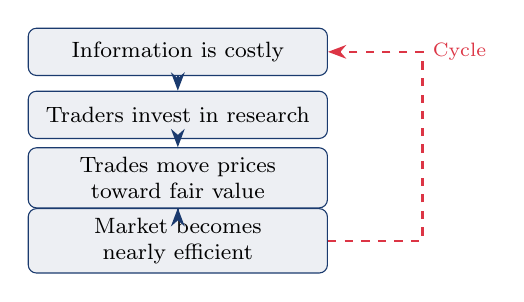
\begin{tikzpicture}[
    every node/.style={font=\small, align=center},
    box/.style={draw=MainBlue, fill=MainBlue!8, rounded corners=3pt,
                minimum width=3.8cm, minimum height=0.6cm, font=\footnotesize}
]
\node[box] (a) at (0,2.4) {Information is costly};
\node[box] (b) at (0,1.6) {Traders invest in research};
\node[box] (c) at (0,0.8) {Trades move prices\\toward fair value};
\node[box] (d) at (0,0) {Market becomes\\nearly efficient};
\draw[-{Stealth}, MainBlue, thick] (a) -- (b);
\draw[-{Stealth}, MainBlue, thick] (b) -- (c);
\draw[-{Stealth}, MainBlue, thick] (c) -- (d);
\draw[-{Stealth}, Crimson, thick, dashed] (d.east) -- ++(1.2,0) |- (a.east) node[midway, right, font=\scriptsize, text=Crimson] {Cycle};
\end{tikzpicture}
\end{center}
\end{column}
\end{columns}
\end{cminipage}
\end{frame}

%#############################################################################
\section{Market Anomalies}
%#############################################################################

\begin{frame}{Calendar Anomalies}
\begin{cminipage}{0.95\textwidth}
\small
\renewcommand{\arraystretch}{1.2}
\begin{center}
\scriptsize
\renewcommand{\arraystretch}{1.3}
\begin{tabular}{lll}
\toprule
\textbf{Anomaly} & \textbf{Description} & \textbf{Current status} \\
\midrule
January effect & Small caps earn more in January & Weakened since discovery \\
Monday effect & Returns lower on Mondays & Largely disappeared \\
Turn-of-month & Higher returns in last/first 3 days & Still present (salary flows) \\
Holiday effect & Higher returns before holidays & Persists weakly \\
Halloween & ``Sell in May and go away'' & Mixed, region-dependent \\
\bottomrule
\end{tabular}
\end{center}

\vspace{0.2cm}
\begin{alertblock}{Publication Bias and Decay}
\begin{itemize}\setlength{\itemsep}{0pt}
    \item Many anomalies weaken or disappear after publication --- consistent with EMH! Arbitrageurs eliminate mispricings once they become known (McLean \& Pontiff, 2016).
\end{itemize}
\end{alertblock}
\end{cminipage}
\end{frame}

\begin{frame}{Cross-Sectional Anomalies}
\begin{cminipage}{0.95\textwidth}
\begin{columns}[T]
\begin{column}{0.48\textwidth}
\begin{block}{Value Effect}
\begin{itemize}\setlength{\itemsep}{0pt}
    \item Stocks with high book-to-market (B/M) earn higher returns (Fama \& French, 1993)
    \item HML factor: $\sim$4\% per year historically
    \item Is it a risk premium or mispricing?
    \item Value stocks are riskier in distress
\end{itemize}
\end{block}

\begin{block}{Size Effect}
\begin{itemize}\setlength{\itemsep}{0pt}
    \item Small-cap stocks earn higher returns (Banz, 1981)
    \item SMB factor: $\sim$2\% per year
    \item Has weakened considerably since discovery
\end{itemize}
\end{block}
\end{column}
\begin{column}{0.48\textwidth}
\begin{block}{Momentum}
\begin{itemize}\setlength{\itemsep}{0pt}
    \item Winners continue to win, losers continue to lose over 3--12 months (Jegadeesh \& Titman, 1993)
    \item WML factor: $\sim$8\% per year
    \item Subject to occasional crashes (2009)
    \item Hardest anomaly to explain rationally
\end{itemize}
\end{block}

\begin{block}{Low Volatility}
\begin{itemize}\setlength{\itemsep}{0pt}
    \item Low-volatility stocks earn higher risk-adjusted returns than high-volatility stocks
    \item Contradicts CAPM's risk-return trade-off
    \item Explanations: leverage constraints, lottery preferences
\end{itemize}
\end{block}
\end{column}
\end{columns}
\end{cminipage}
\end{frame}

\begin{frame}{The Factor Zoo}
\begin{cminipage}{0.95\textwidth}
\begin{itemize}\setlength{\itemsep}{0pt}
    \item Harvey, Liu \& Zhu (2016): over \textbf{300} published factors claimed to predict returns
    \item Many are likely false discoveries due to data mining and $p$-hacking
    \item Hou, Xue \& Zhang (2020): most anomalies do not survive replication with proper corrections
\end{itemize}

\vspace{0.2cm}
\renewcommand{\arraystretch}{1.2}
\begin{center}
\small
\begin{tabular}{lccl}
\toprule
\textbf{Factor} & \textbf{$t$-stat (original)} & \textbf{$t$-stat (replicated)} & \textbf{Status} \\
\midrule
Value (HML) & 3.07 & 2.83 & Robust \\
Momentum (WML) & 4.71 & 3.92 & Robust \\
Size (SMB) & 2.28 & 1.31 & Weakened \\
Accruals & 4.33 & 0.89 & Not robust \\
Asset growth & 5.07 & 1.61 & Weakened \\
\bottomrule
\end{tabular}
\end{center}

\vspace{0.2cm}
\begin{alertblock}{Implication}
\begin{itemize}\setlength{\itemsep}{0pt}
    \item Proper multiple testing corrections (Bonferroni, BH) eliminate most ``anomalies.'' The market may be more efficient than the factor zoo suggests.
\end{itemize}
\end{alertblock}
\end{cminipage}
\end{frame}

%--- Factor Replication ---
\begin{frame}{Factor Replication and Out-of-Sample Decay}
\begin{cminipage}{0.95\textwidth}
\begin{block}{McLean \& Pontiff (2016) --- Key Results}
\begin{itemize}\setlength{\itemsep}{0pt}
    \item Studied 97 published anomalies: average return predictability \textbf{declines 58\%} post-publication
    \item 26\% of the decay is due to statistical overfitting (in-sample bias)
    \item 32\% is due to traders learning and arbitraging away the anomaly
\end{itemize}
\end{block}

\begin{columns}[T]
\begin{column}{0.48\textwidth}
\begin{itemize}\setlength{\itemsep}{0pt}
    \item \textbf{Replication crisis in finance:}
    \item Hou, Xue \& Zhang (2020): 452 anomalies tested; 64\% become insignificant with proper methodology
    \item Multiple testing: with 300 factors tested at 5\%, expect $\sim$15 false discoveries
    \item Adjusted threshold: $t > 3.0$ recommended (Harvey et al., 2016)
\end{itemize}
\end{column}
\begin{column}{0.48\textwidth}
\begin{exampleblock}{EMH Interpretation}
\begin{itemize}\setlength{\itemsep}{0pt}
    \item Anomaly decay is \textbf{exactly what EMH predicts}: once information is public, it gets priced in
    \item Surviving anomalies (value, momentum) may represent \textbf{risk premia}, not mispricing
    \item The boundary between ``risk'' and ``mispricing'' is the central debate in asset pricing
\end{itemize}
\end{exampleblock}
\end{column}
\end{columns}
\end{cminipage}
\end{frame}

%#############################################################################
\section{Behavioral Finance}
%#############################################################################

\begin{frame}{Behavioral Challenges to EMH}
\begin{cminipage}{0.95\textwidth}
\begin{columns}[T]
\begin{column}{0.48\textwidth}
\begin{block}{Cognitive Biases}
\begin{itemize}\setlength{\itemsep}{0pt}
    \item \textbf{Overconfidence:} traders overestimate the precision of their information
    \item \textbf{Anchoring:} prices stick to reference points (52-week high, IPO price)
    \item \textbf{Loss aversion:} losses hurt $\sim$2$\times$ more than equivalent gains (Kahneman \& Tversky, 1979)
    \item \textbf{Herding:} investors follow the crowd, amplifying bubbles and crashes
\end{itemize}
\end{block}
\end{column}
\begin{column}{0.48\textwidth}
\begin{block}{Market-Level Phenomena}
\begin{itemize}\setlength{\itemsep}{0pt}
    \item \textbf{Bubbles:} Tulip mania (1637), Dot-com (2000), US housing (2008), Crypto (2017, 2021)
    \item \textbf{Excess volatility:} Shiller (1981) --- stock prices are more volatile than fundamentals justify
    \item \textbf{Limits to arbitrage:} even if mispricing exists, correcting it is risky and costly (noise trader risk, short-selling constraints)
\end{itemize}
\end{block}
\end{column}
\end{columns}

\vspace{0.2cm}
\begin{exampleblock}{Fama's Counter-Argument}
\begin{itemize}\setlength{\itemsep}{0pt}
    \item Overreaction and underreaction appear equally often $\Rightarrow$ errors are random, not systematic. Anomalies are consistent with the EMH + rational risk premia.
\end{itemize}
\end{exampleblock}
\end{cminipage}
\end{frame}

\begin{frame}{Bubbles and Crashes: A Timeline}
\begin{cminipage}{0.95\textwidth}
\begin{center}
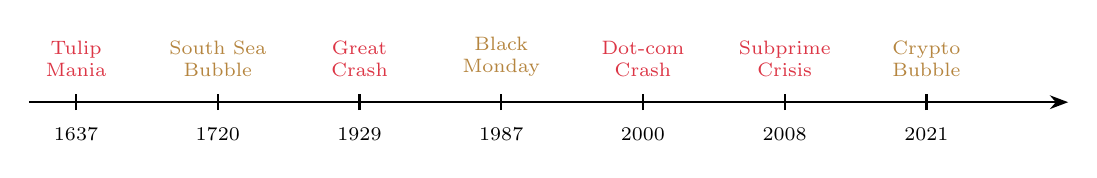
\begin{tikzpicture}[x=0.6cm, y=0.5cm,
    every node/.style={font=\scriptsize, align=center}
]
% Timeline axis
\draw[-{Stealth}, thick] (0,0) -- (22,0);
% Events
\foreach \x/\year/\event in {1/1637/{Tulip\\Mania}, 7/1929/{Great\\Crash}, 13/2000/{Dot-com\\Crash}, 16/2008/{Subprime\\Crisis}} {
    \draw[thick] (\x,-0.2)--(\x,0.2); \node[below=3pt] at (\x,-0.2) {\year};
    \node[above=3pt, text=Crimson] at (\x,0.2) {\event};
}
\foreach \x/\year/\event in {4/1720/{South Sea\\Bubble}, 10/1987/{Black\\Monday}, 19/2021/{Crypto\\Bubble}} {
    \draw[thick] (\x,-0.2)--(\x,0.2); \node[below=3pt] at (\x,-0.2) {\year};
    \node[above=3pt, text=Amber] at (\x,0.2) {\event};
}
\end{tikzpicture}
\end{center}

\vspace{0.3cm}
\begin{itemize}\setlength{\itemsep}{0pt}
    \item \textbf{EMH perspective:} bubbles can only be identified \textit{ex post}; \textit{ex ante}, prices reflected rational expectations given available information
    \item \textbf{Behavioral perspective:} systematic irrationality (herding, speculation) creates predictable patterns
    \item \textbf{Key insight:} even if bubbles exist, it is extremely difficult to profit from them due to timing uncertainty (``the market can stay irrational longer than you can stay solvent'')
\end{itemize}
\end{cminipage}
\end{frame}

%--- Prospect Theory ---
\begin{frame}{Prospect Theory (Kahneman \& Tversky, 1979)}
\begin{cminipage}{0.95\textwidth}
\small
\begin{columns}[T]
\begin{column}{0.48\textwidth}
\begin{block}{Value Function}
\begin{itemize}\setlength{\itemsep}{0pt}
    \item Defined over \textbf{gains and losses} relative to a reference point, not wealth levels:
    $$v(x) = \begin{cases} x^\alpha & x \geq 0 \\ -\lambda(-x)^\beta & x < 0 \end{cases}$$
    \item Typical estimates: $\alpha = \beta \approx 0.88$, $\lambda \approx 2.25$
    \item \textbf{Concave} for gains (risk aversion)
    \item \textbf{Convex} for losses (risk seeking)
    \item \textbf{Steeper} for losses ($\lambda > 1$): loss aversion
\end{itemize}
\end{block}
\end{column}
\begin{column}{0.48\textwidth}
\begin{block}{Probability Weighting}
\begin{itemize}\setlength{\itemsep}{0pt}
    \item Decision weight $w(p) \neq p$:
    $$w(p) = \frac{p^\delta}{(p^\delta + (1-p)^\delta)^{1/\delta}}$$
    \item Overweight small probabilities (lotteries, tail risk)
    \item Underweight moderate-to-high probabilities
    \item Explains: lottery buying, insurance purchasing, and equity premium puzzle
\end{itemize}
\end{block}
\end{column}
\end{columns}

\vspace{0.1cm}
\begin{alertblock}{Implication for EMH}
\begin{itemize}\setlength{\itemsep}{0pt}
    \item If investors evaluate returns via prospect theory (not expected utility), asset prices reflect \textbf{distorted} risk preferences $\Rightarrow$ systematic mispricing
\end{itemize}
\end{alertblock}
\end{cminipage}
\end{frame}

%--- Disposition Effect ---
\begin{frame}{Disposition Effect}
\begin{cminipage}{0.95\textwidth}
\small
\begin{block}{Definition}
\begin{itemize}\setlength{\itemsep}{0pt}
    \item Investors tend to \textbf{sell winners too early} (locking in gains) and \textbf{hold losers too long} (hoping for recovery)
    \item Direct consequence of prospect theory: risk aversion in gains, risk seeking in losses
\end{itemize}
\end{block}

\begin{columns}[T]
\begin{column}{0.48\textwidth}
\begin{itemize}\setlength{\itemsep}{0pt}
    \item \textbf{Odean (1998)} evidence:
    \item Analyzed 10{,}000 brokerage accounts (1987--1993)
    \item Proportion of Gains Realized (PGR) $= 0.148$
    \item Proportion of Losses Realized (PLR) $= 0.098$
    \item PGR/PLR $= 1.51$ $\Rightarrow$ 50\% more likely to sell a winner
\end{itemize}
\end{column}
\begin{column}{0.48\textwidth}
\begin{itemize}\setlength{\itemsep}{0pt}
    \item \textbf{Market implications:}
    \item Stocks with recent gains have excess selling pressure $\Rightarrow$ underpriced
    \item Stocks with recent losses lack selling $\Rightarrow$ overpriced
    \item Contributes to \textbf{momentum}: winners are slow to reach fair value
    \item Tax-loss selling in December partially offsets (but not fully)
\end{itemize}
\end{column}
\end{columns}
\end{cminipage}
\end{frame}

%--- Limits to Arbitrage ---
\begin{frame}{Limits to Arbitrage}
\begin{cminipage}{0.95\textwidth}
\small
\begin{block}{Why Mispricings Persist (DeLong, Shleifer, Summers, Waldmann, 1990)}
\begin{itemize}\setlength{\itemsep}{0pt}
    \item Even if rational arbitrageurs identify mispricing, correcting it is risky and costly
\end{itemize}
\end{block}

\begin{columns}[T]
\begin{column}{0.48\textwidth}
\begin{itemize}\setlength{\itemsep}{0pt}
    \item \textbf{Noise trader risk:} mispricing may worsen before it corrects; arbitrageur faces margin calls
    \item \textbf{Fundamental risk:} no perfect substitute for hedging; idiosyncratic risk remains
    \item \textbf{Synchronization risk:} each arbitrageur waits for others to act first $\Rightarrow$ no one moves
\end{itemize}
\end{column}
\begin{column}{0.48\textwidth}
\begin{itemize}\setlength{\itemsep}{0pt}
    \item \textbf{Short-selling constraints:} borrowing shares is costly, sometimes impossible (``short squeeze'')
    \item \textbf{Model risk:} the apparent mispricing might reflect a missing risk factor
    \item \textbf{Example:} LTCM (1998) --- convergence trades were ``correct'' but blow-up before convergence
\end{itemize}
\end{column}
\end{columns}

\vspace{0.1cm}
\begin{alertblock}{Key Insight}
\begin{itemize}\setlength{\itemsep}{0pt}
    \item Limits to arbitrage explain why markets can be \textbf{informationally inefficient} yet \textbf{not exploitable} --- reconciling EMH with behavioral anomalies
\end{itemize}
\end{alertblock}
\end{cminipage}
\end{frame}

%--- Excess Volatility ---
\begin{frame}{Excess Volatility Puzzle (Shiller, 1981)}
\begin{cminipage}{0.95\textwidth}
\small
\begin{block}{Present Value Model}
\begin{itemize}\setlength{\itemsep}{0pt}
    \item Under EMH, stock price equals discounted future dividends: $P_t = \E_t\left[\sum_{k=1}^{\infty}\frac{D_{t+k}}{(1+r)^k}\right]$
    \item Define the ``ex-post rational price'': $P_t^* = \sum_{k=1}^{\infty}\frac{D_{t+k}}{(1+r)^k}$ (perfect foresight)
    \item Since $P_t = \E_t[P_t^*]$, we must have $\Var(P_t) \leq \Var(P_t^*)$ (variance bound)
\end{itemize}
\end{block}

\begin{columns}[T]
\begin{column}{0.48\textwidth}
\begin{itemize}\setlength{\itemsep}{0pt}
    \item \textbf{Shiller's finding:}
    \item S\&P 500 prices far more volatile than $P_t^*$
    \item $\sigma(P)/\sigma(P^*) \approx 5$--$13$ (depending on period)
    \item Prices ``move too much'' relative to subsequent dividends
\end{itemize}
\end{column}
\begin{column}{0.48\textwidth}
\begin{itemize}\setlength{\itemsep}{0pt}
    \item \textbf{Debate:}
    \item Marsh \& Merton (1986): dividend smoothing biases $P_t^*$
    \item Fama (1991): time-varying risk premia explain excess volatility
    \item Campbell \& Shiller (1988): log-linear model confirms excess volatility
    \item Remains one of the strongest challenges to EMH
\end{itemize}
\end{column}
\end{columns}
\end{cminipage}
\end{frame}

%--- Sentiment Indicators ---
\begin{frame}{Sentiment Indicators}
\begin{cminipage}{0.95\textwidth}
\small
\begin{columns}[T]
\begin{column}{0.48\textwidth}
\begin{block}{Market-Based Indicators}
\begin{itemize}\setlength{\itemsep}{0pt}
    \item \textbf{VIX} (``Fear Index''): implied volatility from S\&P 500 options
    \item High VIX $\Rightarrow$ fear $\Rightarrow$ historically predicts \textbf{higher} future returns
    \item \textbf{Put/Call ratio:} high ratio $=$ bearish sentiment $\Rightarrow$ contrarian buy signal
    \item \textbf{Margin debt:} high margin $\Rightarrow$ euphoria $\Rightarrow$ potential correction
\end{itemize}
\end{block}
\end{column}
\begin{column}{0.48\textwidth}
\begin{block}{Baker--Wurgler Sentiment Index}
\begin{itemize}\setlength{\itemsep}{0pt}
    \item Composite of 6 proxies: closed-end fund discount, NYSE turnover, IPO volume, IPO first-day returns, equity share in new issues, dividend premium
    \item High sentiment $\Rightarrow$ overpricing of speculative stocks
    \item Low sentiment $\Rightarrow$ underpricing of speculative stocks
    \item Predictive for cross-section, not aggregate market
\end{itemize}
\end{block}
\end{column}
\end{columns}

\vspace{0.1cm}
\begin{alertblock}{EMH Interpretation}
\begin{itemize}\setlength{\itemsep}{0pt}
    \item If sentiment predicts returns, prices do not fully reflect available information $\Rightarrow$ challenges semi-strong EMH. However, sentiment-based strategies have limited Sharpe ratios after costs.
\end{itemize}
\end{alertblock}
\end{cminipage}
\end{frame}

%--- Quiz: Behavioral Finance ---
\begin{frame}{Quiz: Behavioral Finance}
\begin{cminipage}{0.95\textwidth}
\small
\begin{alertblock}{Q1}
\begin{itemize}\setlength{\itemsep}{0pt}
    \item Under prospect theory, an investor who is losing 10\% on a stock is most likely to: \textbf{(A)} sell immediately \textbf{(B)} hold and hope for recovery \textbf{(C)} buy more to average down \textbf{(D)} hedge with options
\end{itemize}
\end{alertblock}
\begin{exampleblock}{A1: (B) --- loss aversion makes investors risk-seeking in losses, so they hold losers.}
\end{exampleblock}

\begin{alertblock}{Q2}
\begin{itemize}\setlength{\itemsep}{0pt}
    \item Which is NOT a limit to arbitrage? \textbf{(A)} Noise trader risk \textbf{(B)} Short-selling constraints \textbf{(C)} Diversification \textbf{(D)} Synchronization risk
\end{itemize}
\end{alertblock}
\begin{exampleblock}{A2: (C) --- diversification is a portfolio strategy, not a limit to arbitrage.}
\end{exampleblock}

\begin{alertblock}{Q3}
\begin{itemize}\setlength{\itemsep}{0pt}
    \item Shiller's excess volatility puzzle shows that: \textbf{(A)} dividends are too volatile \textbf{(B)} prices move more than dividends justify \textbf{(C)} volatility is constant \textbf{(D)} CAPM holds exactly
\end{itemize}
\end{alertblock}
\begin{exampleblock}{A3: (B) --- stock prices are far more volatile than the present value of subsequent dividends.}
\end{exampleblock}
\end{cminipage}
\end{frame}

%#############################################################################
\section{The Adaptive Market Hypothesis}
%#############################################################################

\begin{frame}{Andrew Lo's Adaptive Market Hypothesis (2004)}
\begin{cminipage}{0.95\textwidth}
\begin{block}{Core Idea}
\begin{itemize}\setlength{\itemsep}{0pt}
    \item Market efficiency is not a static property but an \textbf{evolving dynamic} driven by evolutionary forces: competition, adaptation, natural selection.
\end{itemize}
\end{block}

\begin{columns}[T]
\begin{column}{0.48\textwidth}
\begin{itemize}\setlength{\itemsep}{0pt}
    \item \textbf{Key principles:}
    \item Investors are neither fully rational nor fully irrational --- they \textbf{adapt}
    \item Market ecology: species (hedge funds, retail, HFT) compete for resources (alpha)
    \item Profit opportunities arise and disappear as strategies become crowded
    \item Risk premia vary over time with market conditions
\end{itemize}
\end{column}
\begin{column}{0.48\textwidth}
\begin{itemize}\setlength{\itemsep}{0pt}
    \item \textbf{Predictions:}
    \item Efficiency varies across markets and time periods
    \item Anomalies appear, attract capital, and then decay
    \item Crises create new inefficiencies (fear, forced selling)
    \item Recovery periods restore efficiency
    \item EMH is a \textbf{limiting case} of AMH when market ecology is stable
\end{itemize}
\end{column}
\end{columns}
\end{cminipage}
\end{frame}

\begin{frame}{EMH vs.\ AMH: A Comparison}
\begin{cminipage}{0.95\textwidth}
\scriptsize
\renewcommand{\arraystretch}{1.3}
\begin{center}
\begin{tabular}{lll}
\toprule
\textbf{Dimension} & \textbf{EMH (Fama)} & \textbf{AMH (Lo)} \\
\midrule
Investor rationality & Fully rational & Boundedly rational, adaptive \\
Market efficiency & Constant & Time-varying, dynamic \\
Risk premia & Constant / slowly varying & Fluctuate with market ecology \\
Anomalies & Statistical artifacts or risk & Real but transient \\
Crises & Rational response to news & Ecological disruptions \\
Investment strategy & Passive (index funds) & Adaptive, regime-dependent \\
Theoretical basis & Neoclassical economics & Evolutionary biology \\
\bottomrule
\end{tabular}
\end{center}

\vspace{0.2cm}
\begin{exampleblock}{Practical Implication}
\begin{itemize}\setlength{\itemsep}{0pt}
    \item Under AMH, the optimal strategy is \textbf{adaptive}: passive in calm periods, active during crises when inefficiencies are greatest.
\end{itemize}
\end{exampleblock}
\end{cminipage}
\end{frame}

\begin{frame}{Measuring Time-Varying Efficiency}
\begin{cminipage}{0.95\textwidth}
\begin{itemize}\setlength{\itemsep}{0pt}
    \item \textbf{Rolling variance ratio:} compute $VR(q)$ over a rolling window (e.g., 500 days)
    \item $|VR(q) - 1|$ as a time-varying \textbf{efficiency index}
    \item During crises (2008, 2020), $|VR - 1|$ spikes $\Rightarrow$ temporary inefficiency
    \item Between crises, $|VR - 1|$ returns to low levels $\Rightarrow$ efficiency is restored
\end{itemize}

\vspace{0.2cm}
\begin{block}{Hurst Exponent as Efficiency Measure}
\begin{columns}[T]
\begin{column}{0.48\textwidth}
\begin{itemize}\setlength{\itemsep}{0pt}
    \item $H = 0.5$: random walk (efficient)
    \item $H > 0.5$: persistence (trending, momentum)
    \item $H < 0.5$: anti-persistence (mean-reverting)
    \item Estimated via R/S analysis or DFA
\end{itemize}
\end{column}
\begin{column}{0.48\textwidth}
\begin{itemize}\setlength{\itemsep}{0pt}
    \item Typical values for daily returns:
    \item S\&P 500: $H \approx 0.52$
    \item BTC-USD: $H \approx 0.55$ (more persistent)
    \item BET: $H \approx 0.58$ (least efficient)
\end{itemize}
\end{column}
\end{columns}
\end{block}
\end{cminipage}
\quantlet{SFM\_ch3\_hurst\_exponent}{https://github.com/QuantLet/Stat_fin_markets/tree/master/Ch_03/SFM_ch3_hurst_exponent}
\end{frame}

\begin{frame}{Hurst Exponent: R/S Analysis Plot}
\begin{cminipage}{0.95\textwidth}
\begin{center}
\IfFileExists{ch3_hurst_exponent.pdf}{%
    
\includegraphics[width=0.55\textwidth]{ch3_hurst_exponent.pdf}
}{%
    \textit{[Chart: R/S analysis --- $\log(R/S)$ vs.\ $\log(n)$ for S\&P 500, BET, BTC --- ch3\_hurst\_exponent.pdf]}
}
\end{center}
\begin{itemize}\setlength{\itemsep}{0pt}
    \item Slope of $\log(R/S)$ vs.\ $\log(n)$ regression estimates the Hurst exponent $H$
    \item $H \approx 0.5$: random walk; $H > 0.5$: long memory; $H < 0.5$: anti-persistence
\end{itemize}
\end{cminipage}
\end{frame}

%--- Code Slide: Hurst Exponent ---
\begin{frame}[fragile]{Python: Hurst Exponent via R/S Analysis}
\begin{cminipage}{0.95\textwidth}
\begin{lstlisting}
import numpy as np, yfinance as yf

sp = yf.download('^GSPC', start='2015-01-01', end='2025-01-01')
r = np.log(sp['Adj Close']/sp['Adj Close'].shift(1)).dropna().values

def hurst_rs(ts, min_w=20, max_w=None):
    """Estimate Hurst exponent via rescaled range."""
    N = len(ts)
    if max_w is None: max_w = N // 4
    wins = [int(w) for w in np.logspace(
                np.log10(min_w), np.log10(max_w), 20)]
    RS = []
    for w in wins:
        rv = []
        for s in range(0, N-w, w):
            seg = ts[s:s+w]; Y = np.cumsum(seg-seg.mean())
            S = seg.std(ddof=1)
            if S > 0: rv.append((Y.max()-Y.min())/S)
        RS.append((w, np.mean(rv)))
    ln, lr = np.log([x[0] for x in RS]), np.log([x[1] for x in RS])
    return np.polyfit(ln, lr, 1)[0]
print(f"Hurst (S&P 500): {hurst_rs(r):.3f}")  # ~0.52
\end{lstlisting}
\end{cminipage}
\quantlet{SFM\_ch3\_hurst\_exponent}{https://github.com/QuantLet/Stat_fin_markets/tree/master/Ch_03/SFM_ch3_hurst_exponent}
\end{frame}

%--- AMH Empirical Evidence ---
\begin{frame}{AMH: Empirical Evidence}
\begin{cminipage}{0.95\textwidth}
\small
\begin{columns}[T]
\begin{column}{0.48\textwidth}
\begin{block}{Time-Varying Sharpe Ratios}
\begin{itemize}\setlength{\itemsep}{0pt}
    \item Rolling 3-year Sharpe ratios for S\&P 500 range from $-0.5$ to $+1.5$
    \item Momentum strategies: SR $> 1$ in 2009--2015, SR $\approx 0$ in 2018--2020
    \item Value strategies: profitable in 2000--2007, underperform in 2010--2020
    \item \textbf{No strategy is permanently profitable} --- consistent with AMH
\end{itemize}
\end{block}
\end{column}
\begin{column}{0.48\textwidth}
\begin{block}{Regime-Dependent Alpha}
\begin{itemize}\setlength{\itemsep}{0pt}
    \item Rolling CAPM alpha for hedge funds varies with VIX regime
    \item Low VIX ($<15$): alpha $\approx 0$ (efficient)
    \item High VIX ($>30$): alpha $\approx 3\%$--$5\%$ annualized
    \item Crisis periods create dislocations that skilled managers exploit
    \item As capital flows in, alpha decays (crowding)
\end{itemize}
\end{block}
\end{column}
\end{columns}

\vspace{0.1cm}
\begin{exampleblock}{Key Takeaway}
\begin{itemize}\setlength{\itemsep}{0pt}
    \item The profitability of trading strategies is \textbf{cyclical}, not permanent --- exactly as AMH predicts
\end{itemize}
\end{exampleblock}
\end{cminipage}
\end{frame}

%--- AMH Investment Implications ---
\begin{frame}{AMH: Investment Implications}
\begin{cminipage}{0.95\textwidth}
\small
\renewcommand{\arraystretch}{1.2}
\begin{center}
\footnotesize
\begin{tabular}{lll}
\toprule
\textbf{Market Regime} & \textbf{Optimal Strategy} & \textbf{Rationale} \\
\midrule
Low volatility, trending & Passive indexing & Markets are efficient; alpha $\approx 0$ \\
High volatility, crisis & Active/tactical & Dislocations create opportunities \\
Post-crisis recovery & Momentum overweight & Mean reversion from overshooting \\
Crowded factor regime & Factor diversification & Single factors lose edge \\
Structural change & Adaptive rebalancing & Old relationships break down \\
\bottomrule
\end{tabular}
\end{center}

\vspace{0.2cm}
\begin{columns}[T]
\begin{column}{0.48\textwidth}
\begin{itemize}\setlength{\itemsep}{0pt}
    \item \textbf{Risk parity adaptation:} equal risk contribution works in calm periods; shift to defensive in crises
    \item \textbf{Factor timing:} rotate between value, momentum, quality based on macro regime
\end{itemize}
\end{column}
\begin{column}{0.48\textwidth}
\begin{itemize}\setlength{\itemsep}{0pt}
    \item \textbf{Practical rule:} be passive by default, active only when opportunity cost of passivity is high
    \item \textbf{Monitoring signal:} $|VR(q) - 1|$ spike $\Rightarrow$ potential for active alpha
\end{itemize}
\end{column}
\end{columns}
\end{cminipage}
\end{frame}

%--- AMH vs FMH ---
\begin{frame}{AMH vs Fractal Market Hypothesis}
\begin{cminipage}{0.95\textwidth}
\small
\begin{columns}[T]
\begin{column}{0.48\textwidth}
\begin{block}{Fractal Market Hypothesis (Peters, 1994)}
\begin{itemize}\setlength{\itemsep}{0pt}
    \item Markets are stable when investors with \textbf{different time horizons} participate
    \item Short-horizon traders provide liquidity to long-horizon investors
    \item Crises occur when all horizons \textbf{synchronize} (everyone sells)
    \item Multi-fractal models: $\text{MF-DFA}$, $\text{MF-DCCA}$
\end{itemize}
\end{block}
\end{column}
\begin{column}{0.48\textwidth}
\begin{block}{Comparison}
\footnotesize
\renewcommand{\arraystretch}{1.1}
\begin{tabular}{lll}
\toprule
& \textbf{AMH} & \textbf{FMH} \\
\midrule
Basis & Evolution & Fractals \\
Key driver & Adaptation & Time horizons \\
Crises & Ecological & Horizon collapse \\
Math tool & Rolling tests & MF-DFA \\
Efficiency & Time-varying & Scale-dependent \\
\bottomrule
\end{tabular}
\end{block}
\end{column}
\end{columns}

\vspace{0.1cm}
\begin{alertblock}{Mandelbrot's Legacy}
\begin{itemize}\setlength{\itemsep}{0pt}
    \item Both AMH and FMH reject the assumption of constant market dynamics; they differ in mechanism (biological adaptation vs.\ mathematical self-similarity) but agree that EMH is a special case
\end{itemize}
\end{alertblock}
\end{cminipage}
\end{frame}

%--- Market Ecology ---
\begin{frame}{Market Ecology}
\begin{cminipage}{0.95\textwidth}
\small
\begin{block}{Lo's Species Analogy}
\begin{itemize}\setlength{\itemsep}{0pt}
    \item Market participants as ``species'' competing for alpha (``food'')
    \item When a niche is overcrowded, returns shrink $\Rightarrow$ weaker species exit
\end{itemize}
\end{block}

\footnotesize
\renewcommand{\arraystretch}{1.1}
\begin{center}
\begin{tabular}{lll}
\toprule
\textbf{Species} & \textbf{Strategy} & \textbf{Impact on Efficiency} \\
\midrule
Retail investors & Buy-and-hold, sentiment-driven & Provide noise, reduce efficiency \\
Hedge funds & Factor-based, arbitrage & Increase efficiency (correct mispricing) \\
HFT firms & Market-making, latency arb & Improve short-term efficiency \\
Index funds & Passive replication & Price-takers; no information role \\
Dark pools & Off-exchange matching & Reduce transparency, mixed effect \\
\bottomrule
\end{tabular}
\end{center}

\vspace{0.1cm}
\begin{itemize}\setlength{\itemsep}{0pt}
    \item \textbf{HFT debate:} improves liquidity and narrows spreads, but ``phantom liquidity'' disappears in crises
    \item \textbf{Dark pools:} $\sim$40\% of US equity volume; reduce information leakage but fragment price discovery
    \item \textbf{Passive investing growth:} if too many are passive, who corrects mispricing? (Grossman--Stiglitz paradox revisited)
\end{itemize}
\end{cminipage}
\end{frame}

%#############################################################################
\section{Case Study: S\&P 500 EMH Analysis}
%#############################################################################

\begin{frame}{Efficiency Comparison Across Markets}
\begin{cminipage}{0.95\textwidth}
\begin{center}
\IfFileExists{ch3_efficiency_comparison.pdf}{%
    
\includegraphics[width=0.55\textwidth]{ch3_efficiency_comparison.pdf}
}{%
    \textit{[Chart: Efficiency comparison across developed vs.\ emerging markets --- ch3\_efficiency\_comparison.pdf]}
}
\end{center}
\begin{itemize}\setlength{\itemsep}{0pt}
    \item Efficiency indicators (VR, Hurst, autocorrelation) compared for S\&P 500, FTSE 100, BET, BTC-USD
    \item Developed markets are closer to weak-form efficiency
    \item Emerging markets show significant deviations, especially at longer horizons
\end{itemize}
\end{cminipage}
\end{frame}

\begin{frame}{Case Study: Comprehensive EMH Testing on S\&P 500}
\begin{cminipage}{0.95\textwidth}
\small
\begin{block}{Setup}
\begin{itemize}\setlength{\itemsep}{0pt}
    \item Data: S\&P 500 daily log-returns, Jan 2000 -- Dec 2024 ($T \approx 6{,}300$)
    \item Goal: apply all weak-form tests and interpret jointly
\end{itemize}
\end{block}

\vspace{0.1cm}
\scriptsize
\renewcommand{\arraystretch}{1.1}
\begin{center}
\begin{tabular}{llll}
\toprule
\textbf{Test} & \textbf{Statistic} & \textbf{$p$-value} & \textbf{Decision at 5\%} \\
\midrule
Ljung--Box $Q(10)$ & 15.3 & 0.12 & Do not reject \\
Ljung--Box $Q(20)$ & 28.1 & 0.11 & Do not reject \\
Runs test & $Z = -1.42$ & 0.16 & Do not reject \\
VR(2) & 1.047 ($z = 1.88$) & 0.06 & Do not reject (marginal) \\
VR(5) & 1.038 ($z = 1.21$) & 0.23 & Do not reject \\
VR(10) & 0.993 ($z = -0.18$) & 0.86 & Do not reject \\
ADF (prices) & $-1.85$ & 0.35 & Do not reject (unit root) \\
ADF (returns) & $-52.3$ & $<0.001$ & Reject (stationary) \\
Hurst exponent & $H = 0.523$ & --- & Near 0.5 (efficient) \\
\bottomrule
\end{tabular}
\end{center}
\end{cminipage}
\quantlet{SFM\_ch3\_emh\_tests}{https://github.com/QuantLet/Stat_fin_markets/tree/master/Ch_03/SFM_ch3_emh_tests}
\end{frame}

\begin{frame}{Case Study: Interpretation and Conclusions}
\begin{cminipage}{0.95\textwidth}
\small
\begin{columns}[T]
\begin{column}{0.48\textwidth}
\begin{block}{Findings}
\begin{itemize}\setlength{\itemsep}{0pt}
    \item All tests fail to reject weak-form EMH at 5\%
    \item $VR(2)$ is marginally significant --- small positive autocorrelation at lag 1
    \item $H = 0.523 \approx 0.5$ $\Rightarrow$ mild persistence
    \item Prices: unit root; returns: stationary
\end{itemize}
\end{block}
\end{column}
\begin{column}{0.48\textwidth}
\begin{alertblock}{Caveats}
\begin{itemize}\setlength{\itemsep}{0pt}
    \item $\hat{\rho}_1 \approx 0.05$ is significant with $T = 6{,}300$ but generates $< 0.1\%$ daily $\Rightarrow$ consumed by costs
    \item Joint hypothesis: we assume CAPM
    \item Subperiods around crises may reject
    \item $|r_t|$ is autocorrelated $\Rightarrow$ volatility is predictable, returns are not
\end{itemize}
\end{alertblock}
\end{column}
\end{columns}

\vspace{0.1cm}
\begin{exampleblock}{Bottom Line}
\begin{itemize}\setlength{\itemsep}{0pt}
    \item The S\&P 500 is approximately weak-form efficient. Small statistical deviations exist but are not economically exploitable after costs.
\end{itemize}
\end{exampleblock}
\end{cminipage}
\end{frame}

%--- Case Study: Bitcoin ---
\begin{frame}{Case Study: Bitcoin Efficiency}
\begin{cminipage}{0.95\textwidth}
\small
\begin{block}{Evolution of BTC-USD Efficiency (2015--2024)}
\begin{itemize}\setlength{\itemsep}{0pt}
    \item Bitcoin has transitioned from a clearly inefficient market to one approaching weak-form efficiency
\end{itemize}
\end{block}

\footnotesize
\renewcommand{\arraystretch}{1.1}
\begin{center}
\begin{tabular}{llllll}
\toprule
\textbf{Period} & \textbf{LB(10) $p$} & \textbf{$VR(5)$} & \textbf{$\hat{H}$} & \textbf{Daily vol} & \textbf{Efficiency} \\
\midrule
2015--2016 & 0.001 & 1.22 & 0.62 & 4.2\% & \textcolor{Crimson}{Inefficient} \\
2017 (bubble) & 0.003 & 1.35 & 0.68 & 5.8\% & \textcolor{Crimson}{Inefficient} \\
2018--2019 & 0.04 & 1.12 & 0.57 & 3.9\% & \textcolor{Amber}{Marginal} \\
2020--2021 & 0.08 & 1.08 & 0.55 & 3.5\% & \textcolor{Amber}{Marginal} \\
2022--2024 & 0.18 & 1.04 & 0.53 & 2.8\% & \textcolor{Forest}{Near-efficient} \\
\bottomrule
\end{tabular}
\end{center}

\vspace{0.1cm}
\begin{itemize}\setlength{\itemsep}{0pt}
    \item \textbf{Early period:} thin liquidity, retail-dominated, strong momentum $\Rightarrow$ high $H$, significant autocorrelation
    \item \textbf{Maturation:} institutional entry (CME futures 2017, ETFs 2024), increased liquidity, algorithmic trading
    \item \textbf{Current state:} daily returns approximately efficient; intraday still shows microstructure patterns
\end{itemize}
\end{cminipage}
\end{frame}

%--- Case Study: BET ---
\begin{frame}{Case Study: Bucharest Stock Exchange (BET)}
\begin{cminipage}{0.95\textwidth}
\small
\begin{columns}[T]
\begin{column}{0.48\textwidth}
\begin{block}{BET Efficiency Results}
\footnotesize
\renewcommand{\arraystretch}{1.1}
\begin{tabular}{ll}
\toprule
\textbf{Test} & \textbf{Result} \\
\midrule
LB(10) $p$-value & $<0.01$ \\
$VR(5)$ & 1.18 ($z = 3.2$) \\
$\hat{H}$ (R/S) & 0.58 \\
ADF (returns) $p$ & $<0.001$ \\
$\hat{\rho}_1$ & 0.12 \\
\bottomrule
\end{tabular}
\end{block}
\begin{itemize}\setlength{\itemsep}{0pt}
    \item Significant autocorrelation: $\hat{\rho}_1 = 0.12$
    \item $VR(5) = 1.18 \gg 1$: strong momentum
    \item $H = 0.58$: persistent, inefficient
\end{itemize}
\end{column}
\begin{column}{0.48\textwidth}
\begin{alertblock}{Why Less Efficient?}
\begin{itemize}\setlength{\itemsep}{0pt}
    \item Low liquidity: avg daily turnover $\sim$\EUR{10M}
    \item Few institutional investors
    \item Limited analyst coverage
    \item Information asymmetry between insiders and retail
    \item Thin order books $\Rightarrow$ large bid-ask spreads
\end{itemize}
\end{alertblock}
\begin{exampleblock}{Implications}
\begin{itemize}\setlength{\itemsep}{0pt}
    \item Momentum strategies may work \textit{before} costs
    \item High transaction costs offset predictability
    \item EU accession improved efficiency over time
\end{itemize}
\end{exampleblock}
\end{column}
\end{columns}
\end{cminipage}
\end{frame}

%--- Case Study: Gold ---
\begin{frame}{Case Study: Gold as Safe Haven}
\begin{cminipage}{0.95\textwidth}
\small
\begin{columns}[T]
\begin{column}{0.48\textwidth}
\begin{block}{Gold Returns Properties}
\begin{itemize}\setlength{\itemsep}{0pt}
    \item Daily returns: $\mu \approx 0.03\%$, $\sigma \approx 1.0\%$
    \item Skewness: $-0.15$ (slight left skew)
    \item Kurtosis: 7.2 (fat tails)
    \item Low correlation with equities ($\rho \approx -0.05$)
\end{itemize}
\end{block}
\begin{block}{Efficiency Tests}
\footnotesize
\renewcommand{\arraystretch}{1.1}
\begin{tabular}{ll}
\toprule
\textbf{Test} & \textbf{Result} \\
\midrule
LB(10) $p$ & 0.35 \\
$VR(5)$ & 0.97 \\
$\hat{H}$ & 0.49 \\
\bottomrule
\end{tabular}
\end{block}
\end{column}
\begin{column}{0.48\textwidth}
\begin{itemize}\setlength{\itemsep}{0pt}
    \item $VR(5) = 0.97 < 1$: slight mean reversion
    \item $H = 0.49 < 0.5$: anti-persistent
    \item Gold is highly liquid (24/7 OTC market) $\Rightarrow$ near-efficient
    \item \textbf{Safe haven property:} negative correlation with equities during crises (2008, 2020)
    \item \textbf{Mean reversion:} gold tends to revert to production cost / inflation-adjusted mean
    \item Not a pure random walk, but efficient in practice (deviations too small to exploit)
\end{itemize}
\end{column}
\end{columns}
\end{cminipage}
\end{frame}

%--- Cross-Asset Ranking ---
\begin{frame}{Cross-Asset Efficiency Ranking}
\begin{cminipage}{0.95\textwidth}
\small
\begin{center}
\footnotesize
\renewcommand{\arraystretch}{1.2}
\begin{tabular}{llllll}
\toprule
\textbf{Rank} & \textbf{Asset} & \textbf{$|VR(5)-1|$} & \textbf{$|\hat{H}-0.5|$} & \textbf{$|\hat{\rho}_1|$} & \textbf{Efficiency Score} \\
\midrule
1 & EUR/USD (FX) & 0.01 & 0.01 & 0.01 & 0.99 \\
2 & S\&P 500 & 0.04 & 0.02 & 0.05 & 0.96 \\
3 & Gold (XAU) & 0.03 & 0.01 & 0.03 & 0.97 \\
4 & US 10Y Treasury & 0.05 & 0.03 & 0.04 & 0.95 \\
5 & BTC-USD & 0.04 & 0.03 & 0.05 & 0.95 \\
6 & BSE Sensex & 0.08 & 0.04 & 0.07 & 0.90 \\
7 & BET (Romania) & 0.18 & 0.08 & 0.12 & 0.80 \\
8 & SSE (China) & 0.15 & 0.07 & 0.10 & 0.83 \\
\bottomrule
\end{tabular}
\end{center}

\vspace{0.1cm}
\begin{itemize}\setlength{\itemsep}{0pt}
    \item \textbf{Efficiency score:} $1 - \frac{1}{3}(|VR-1| + 2|\hat{H}-0.5| + |\hat{\rho}_1|)$, normalized to $[0,1]$
    \item FX markets are most efficient: highest liquidity, 24-hour trading, most participants
    \item Emerging equity markets are least efficient: lower liquidity, fewer analysts, more retail
    \item BTC has improved dramatically; now comparable to developed market equities
\end{itemize}
\end{cminipage}
\end{frame}

%--- Event Study: AAPL ---
\begin{frame}{Event Study: AAPL Earnings Announcement}
\begin{cminipage}{0.95\textwidth}
\small
\begin{center}
\IfFileExists{ch3_event_study.pdf}{%
    
\includegraphics[width=0.50\textwidth]{ch3_event_study.pdf}
}{%
    \textit{[Chart: Event study CAR around AAPL earnings --- ch3\_event\_study.pdf]}
}
\end{center}
\begin{itemize}\setlength{\itemsep}{0pt}
    \item \textbf{Event:} Apple Q4 2024 earnings beat ($+$8\% EPS surprise)
    \item $\overline{AR}_0 = +3.2\%$ on announcement day (statistically significant, $t = 4.8$)
    \item $\overline{CAR}(-1, +1) = +4.1\%$: most adjustment within 1 day
    \item $\overline{CAR}(+2, +20) = +0.8\%$: small post-event drift (mild PEAD)
    \item \textbf{Interpretation:} mostly consistent with semi-strong EMH; the bulk of adjustment is immediate, with only a small residual drift
\end{itemize}
\end{cminipage}
\end{frame}

%--- Time-Varying Efficiency ---
\begin{frame}{Time-Varying Efficiency: Evidence}
\begin{cminipage}{0.95\textwidth}
\small
\begin{center}
\IfFileExists{ch3_variance_ratio.pdf}{%
    
\includegraphics[width=0.50\textwidth]{ch3_variance_ratio.pdf}
}{%
    \textit{[Chart: Rolling VR and Hurst exponent --- ch3\_variance\_ratio.pdf]}
}
\end{center}
\begin{itemize}\setlength{\itemsep}{0pt}
    \item Rolling $|VR(5) - 1|$ (500-day window) for S\&P 500 spikes during crises:
    \item \textbf{GFC (2008--09):} $|VR - 1| \approx 0.12$ --- autocorrelation from panic selling, forced liquidation
    \item \textbf{COVID (2020):} $|VR - 1| \approx 0.08$ --- brief inefficiency, rapid recovery
    \item \textbf{Calm periods:} $|VR - 1| < 0.03$ --- near-perfect random walk
    \item \textbf{Rolling $H$:} spikes to $\sim$0.60 during crises (persistence), returns to $\sim$0.52 in calm periods
    \item Crisis-driven inefficiency creates \textbf{temporary alpha opportunities} for adaptive investors (AMH)
\end{itemize}
\end{cminipage}
\end{frame}

%--- Market Microstructure ---
\begin{frame}{Efficiency and Market Microstructure}
\begin{cminipage}{0.95\textwidth}
\small
\begin{columns}[T]
\begin{column}{0.48\textwidth}
\begin{block}{Microstructure Effects on Tests}
\begin{itemize}\setlength{\itemsep}{0pt}
    \item \textbf{Bid-ask bounce:} trade prices alternate between bid and ask $\Rightarrow$ negative autocorrelation ($\hat{\rho}_1 < 0$) even if true returns are i.i.d.
    \item Roll (1984): $\hat{\rho}_1 \approx -s^2/4$ where $s$ is the spread
    \item \textbf{Non-synchronous trading:} illiquid stocks update prices with delay $\Rightarrow$ spurious cross-autocorrelation
\end{itemize}
\end{block}
\end{column}
\begin{column}{0.48\textwidth}
\begin{alertblock}{Epps Effect}
\begin{itemize}\setlength{\itemsep}{0pt}
    \item Correlations between assets \textbf{decrease} as sampling frequency increases
    \item At 1-min: $\rho \approx 0.15$; at daily: $\rho \approx 0.50$
    \item Caused by non-synchronous arrivals of information
    \item Implication: high-frequency tests of EMH are contaminated by microstructure noise
\end{itemize}
\end{alertblock}
\begin{exampleblock}{Practical Rule}
\begin{itemize}\setlength{\itemsep}{0pt}
    \item Use daily or lower frequency for EMH tests to avoid microstructure artifacts
\end{itemize}
\end{exampleblock}
\end{column}
\end{columns}
\end{cminipage}
\end{frame}

%#############################################################################
\section{Conclusions and References}
%#############################################################################

\begin{frame}{Summary: The State of EMH}
\begin{cminipage}{0.95\textwidth}
\begin{columns}[T]
\begin{column}{0.48\textwidth}
\begin{block}{What the evidence supports}
\begin{itemize}\setlength{\itemsep}{0pt}
    \item Most actively managed funds \textbf{underperform} passive benchmarks
    \item Many anomalies \textbf{decay} after publication
    \item Short-term price prediction is extremely difficult
    \item Transaction costs eliminate most trading profits
\end{itemize}
\end{block}
\end{column}
\begin{column}{0.48\textwidth}
\begin{block}{What challenges EMH}
\begin{itemize}\setlength{\itemsep}{0pt}
    \item Momentum and value effects persist
    \item PEAD is robust across markets
    \item Insider trading is profitable
    \item Bubbles and crashes occur periodically
    \item Market efficiency varies over time
\end{itemize}
\end{block}
\end{column}
\end{columns}

\vspace{0.3cm}
\begin{alertblock}{Practical Takeaway}
\begin{itemize}\setlength{\itemsep}{0pt}
    \item Markets are ``efficiently inefficient'' (Pedersen, 2015): efficient enough that most cannot beat them, but with enough friction to reward sophisticated, informed investors.
\end{itemize}
\end{alertblock}
\end{cminipage}
\end{frame}

%--- AI Exercise ---
\begin{frame}[shrink=3]{AI Exercise: Testing Market Efficiency}
    \begin{cminipage}{0.95\textwidth}
    \begin{block}{\footnotesize Prompt to test in ChatGPT / Claude / Copilot}
        {\small
        ``Download daily data for S\&P~500 from 2015 to 2025 using Python (\texttt{yfinance}).
        Compute log-returns. Test the weak-form EMH using: (1) Ljung--Box test on the first 20 lags,
        (2) Lo--MacKinlay variance ratio test for $q = 2, 5, 10, 20$,
        (3) Hurst exponent via R/S analysis,
        (4) ADF unit root test on both prices and returns.
        Interpret each result. Is the S\&P~500 weak-form efficient?''}
    \end{block}
    \vspace{-1mm}
    {\small
    \textbf{Exercise}:
    \begin{enumerate}
        \item Does the AI compute log-returns correctly? Check: $r_t = \ln(P_t / P_{t-1})$, not simple returns
        \item Is the Ljung--Box test applied to \textbf{returns} (not prices)? Does it use the correct $\chi^2(m)$ distribution?
        \item Does the variance ratio correctly use $VR(q) = \Var(r_t(q))/(q \cdot \Var(r_t))$? Check the formula
        \item Is the Hurst exponent computed via R/S or DFA? Is $H \approx 0.5$ interpreted as efficient?
        \item Does the AI distinguish between \textbf{statistical} and \textbf{economic} significance?
        \item Ask: ``What if I test BET (Romania) instead?'' Does the AI recognize emerging market differences?
    \end{enumerate}
    }
    \vspace{-1mm}
    \begin{alertblock}{}
        {\small
        \begin{itemize}\setlength{\itemsep}{0pt}
            \item \textbf{Warning}: AI often applies the ADF test to \textit{returns} and concludes ``no unit root = efficient.'' This is wrong --- the ADF on returns tests stationarity, not efficiency. The relevant test is on \textit{prices}.
        \end{itemize}
        }
    \end{alertblock}
    \end{cminipage}
\end{frame}

%#############################################################################
\section{Quiz}
%#############################################################################

\begin{frame}{Question 1}
    \begin{cminipage}{0.95\textwidth}
    \begin{alertblock}{Question}
        \begin{itemize}
            \item A researcher computes the Ljung--Box statistic $Q(10) = 18.5$ for daily S\&P~500 returns. The critical value $\chi^2_{10, 0.05} = 18.31$. What is the conclusion?
        \end{itemize}
    \end{alertblock}

    \vspace{0.3cm}

    \begin{block}{Answer choices}
        \begin{itemize}\setlength{\itemsep}{2pt}
        \item \textcolor{MainBlue}{\textbf{(A)}} Reject weak-form EMH: returns are autocorrelated
        \item \textcolor{MainBlue}{\textbf{(B)}} Do not reject EMH: the test is inconclusive
        \item \textcolor{MainBlue}{\textbf{(C)}} Reject strong-form EMH
        \item \textcolor{MainBlue}{\textbf{(D)}} Cannot decide without the variance ratio
        \end{itemize}
    \end{block}
    \end{cminipage}
\end{frame}

\begin{frame}{Question 1: Answer}
    \begin{cminipage}{0.95\textwidth}
    \begin{exampleblock}{Answer: (A)}
    \begin{itemize}\setlength\itemsep{1pt}
        \item Since $Q(10) = 18.5 > 18.31 = \chi^2_{10, 0.05}$, we reject $H_0$ at 5\%.
        \item $H_0$: $\rho_1 = \cdots = \rho_{10} = 0$ (returns are uncorrelated).
        \item Rejection means returns have statistically significant autocorrelation $\Rightarrow$ challenges weak-form EMH.
        \item \textbf{Caveat}: statistical significance $\neq$ economic significance. The autocorrelations may be too small to exploit profitably after transaction costs.
        \item (B) is wrong: $Q > \chi^2_{\text{crit}}$ $\Rightarrow$ we \textit{do} reject. (C) is wrong: Ljung--Box tests weak-form, not strong-form.
    \end{itemize}
    \end{exampleblock}
    \end{cminipage}
\end{frame}

\begin{frame}{Question 2}
    \begin{cminipage}{0.95\textwidth}
    \begin{alertblock}{Question}
        \begin{itemize}
            \item A market has Hurst exponent $H = 0.65$. This implies:
        \end{itemize}
    \end{alertblock}

    \vspace{0.3cm}

    \begin{block}{Answer choices}
        \begin{itemize}\setlength{\itemsep}{2pt}
        \item \textcolor{MainBlue}{\textbf{(A)}} Returns are anti-persistent (mean-reverting)
        \item \textcolor{MainBlue}{\textbf{(B)}} Returns are consistent with a random walk
        \item \textcolor{MainBlue}{\textbf{(C)}} Returns are persistent (trending behavior)
        \item \textcolor{MainBlue}{\textbf{(D)}} The market is strong-form efficient
        \end{itemize}
    \end{block}
    \end{cminipage}
\end{frame}

\begin{frame}{Question 2: Answer}
    \begin{cminipage}{0.95\textwidth}
    \begin{exampleblock}{Answer: (C)}
    \begin{itemize}
        \item $H > 0.5$ indicates persistent behavior: positive returns tend to follow positive returns (and vice versa).
        \item $H = 0.5$: random walk (no memory). $H < 0.5$: anti-persistent (mean-reverting). $H > 0.5$: persistent (trending).
        \item $H = 0.65$ is well above 0.5, suggesting significant long-range dependence.
        \item This challenges weak-form EMH: past returns contain information about future returns.
        \item (A) would require $H < 0.5$. (B) requires $H = 0.5$. (D) is unrelated to the Hurst exponent.
    \end{itemize}
    \end{exampleblock}
    \end{cminipage}
\end{frame}

\begin{frame}{Question 3: Reasoning --- Event Study Interpretation}
    \begin{cminipage}{0.95\textwidth}
    \begin{alertblock}{Question}
        \begin{itemize}
            \item After a positive earnings surprise, a stock's CAR drifts upward by 2\% over the following 60 days. This is evidence against:
        \end{itemize}
    \end{alertblock}

    \vspace{0.3cm}

    \begin{block}{Answer choices}
        \begin{itemize}\setlength{\itemsep}{2pt}
        \item \textcolor{MainBlue}{\textbf{(A)}} Weak-form efficiency only
        \item \textcolor{MainBlue}{\textbf{(B)}} Semi-strong efficiency (the information was public)
        \item \textcolor{MainBlue}{\textbf{(C)}} Strong-form efficiency only
        \item \textcolor{MainBlue}{\textbf{(D)}} No form of efficiency --- anomalies are always explained by risk
        \end{itemize}
    \end{block}
    \end{cminipage}
\end{frame}

\begin{frame}{Question 3: Answer}
    \begin{cminipage}{0.95\textwidth}
    \begin{exampleblock}{Answer: (B)}
    \begin{itemize}
        \item Earnings announcements are \textbf{public information}. If the market is semi-strong efficient, prices should adjust immediately and completely.
        \item A 60-day drift after the announcement means the market \textbf{underreacts} to public information $\Rightarrow$ violation of semi-strong EMH.
        \item This is the Post-Earnings Announcement Drift (PEAD), one of the most robust anomalies.
        \item (A) is incomplete: PEAD uses public info, not just past prices. (C) is wrong: insider info is not involved.
        \item (D) is Fama's counter-argument, but the drift pattern is systematic and one-directional.
    \end{itemize}
    \end{exampleblock}
    \end{cminipage}
\end{frame}

%#############################################################################
\section{Exam Exercises}
%#############################################################################

\begin{frame}{Exercise 1: Ljung--Box Test and Weak-Form EMH}
\begin{block}{Problem}
\begin{itemize}
\item A researcher computes the following sample autocorrelations from $T = 500$ daily stock returns:
\end{itemize}
\begin{center}
{\small
\renewcommand{\arraystretch}{1.2}
\begin{tabular}{lcccccc}
\toprule
Lag $k$ & 1 & 2 & 3 & 4 & 5 \\
\midrule
$\hat{\rho}_k$ & 0.08 & $-0.03$ & 0.05 & 0.02 & $-0.01$ \\
\bottomrule
\end{tabular}
}
\end{center}
\end{block}
\begin{enumerate}
    \item Compute the Ljung--Box statistic: $Q(5) = T(T+2)\sum_{k=1}^{5}\frac{\hat{\rho}_k^2}{T-k}$
    \item Compare $Q(5)$ with $\chi^2_5(0.05) = 11.07$. Is weak-form EMH rejected?
    \item Is $\hat{\rho}_1 = 0.08$ individually significant? (Use $z_{\alpha/2}/\sqrt{T}$ with $z_{0.025} = 1.96$)
    \item Discuss: if $\hat{\rho}_1$ is significant but $Q(5)$ is not, what does this mean economically?
\end{enumerate}
\end{frame}

\begin{frame}{Exercise 2: Variance Ratio Test}
\begin{block}{Problem}
\begin{itemize}
\item For a stock index, you estimate: $\hat{\sigma}^2(r_t) = 0.0001$ (daily variance) and $\hat{\sigma}^2(r_t(5)) = 0.00058$ (5-day return variance), with $T = 1{,}000$ observations.
\end{itemize}
\end{block}
\begin{enumerate}
    \item Compute $VR(5) = \hat{\sigma}^2(r_t(5)) / (5 \cdot \hat{\sigma}^2(r_t))$
    \item Is $VR(5) > 1$ or $< 1$? Interpret in terms of autocorrelation (momentum vs.\ mean reversion)
    \item Compute the asymptotic variance under homoscedasticity: $\phi(5) = \frac{2(2 \cdot 5 - 1)(5 - 1)}{3 \cdot 5 \cdot T}$
    \item Compute the $z$-statistic: $z = (VR(5) - 1)/\sqrt{\phi(5)}$. Is the random walk rejected at 5\%?
\end{enumerate}
\vspace{0.1cm}
\begin{exampleblock}{Hint}
$z_{0.025} = 1.96$. Reject $H_0$ (random walk) if $|z| > 1.96$.
\end{exampleblock}
\end{frame}

\begin{frame}{Exercise 3: Event Study}
\begin{block}{Problem}
\begin{itemize}
\item An event study examines $N = 30$ firms around earnings announcements. Market model parameters: $\hat{\alpha} = 0.001$, $\hat{\beta} = 1.2$. On the event day:
\end{itemize}
\begin{center}
{\small
\renewcommand{\arraystretch}{1.2}
\begin{tabular}{lcc}
\toprule
& \textbf{Firm return $R_i$} & \textbf{Market return $R_m$} \\
\midrule
Average across 30 firms & 2.5\% & 0.3\% \\
\bottomrule
\end{tabular}
}
\end{center}
\end{block}
\begin{enumerate}
    \item Compute the average abnormal return: $\overline{AR} = \bar{R}_i - (\hat{\alpha} + \hat{\beta}\bar{R}_m)$
    \item If the standard deviation of $AR_i$ across firms is $\hat{\sigma}_{AR} = 1.8\%$, compute the $t$-statistic: $t = \overline{AR} / (\hat{\sigma}_{AR}/\sqrt{N})$
    \item Is the abnormal return significant at 5\% ($t_{0.025, 29} \approx 2.045$)?
    \item If the $\overline{CAR}(-10, +10) = 3.2\%$ with $\hat{\sigma}_{CAR} = 4.5\%$, is the cumulative effect significant?
\end{enumerate}
\end{frame}

%--- Exercise 4: ADF ---
\begin{frame}{Exercise 4: ADF Test Interpretation}
\begin{block}{Problem}
\begin{itemize}
\item A researcher applies the ADF test (with constant, no trend) to daily log-prices of a stock index with $T = 2{,}000$ observations. The results are:
\end{itemize}
\begin{center}
{\small
\renewcommand{\arraystretch}{1.2}
\begin{tabular}{ll}
\toprule
ADF statistic (prices) & $-2.15$ \\
ADF statistic (returns) & $-38.7$ \\
Critical value (5\%, no trend) & $-2.86$ \\
Optimal lag (BIC) & $p = 3$ \\
\bottomrule
\end{tabular}
}
\end{center}
\end{block}
\begin{enumerate}
    \item Is there a unit root in log-prices? Compare the test statistic with the critical value.
    \item Are log-returns stationary? Interpret the ADF on returns.
    \item What does this jointly imply about weak-form EMH?
    \item If the KPSS test on prices gives statistic $= 0.52$ with 5\% critical value $= 0.146$, does this confirm or contradict the ADF result?
\end{enumerate}
\end{frame}

%--- Exercise 5: Filter Rule ---
\begin{frame}{Exercise 5: Filter Rule Profitability}
\begin{block}{Problem}
\begin{itemize}
\item A stock has the following daily prices over 10 days: 100, 101.5, 100.8, 99.5, 100.2, 101.8, 103.0, 102.1, 100.5, 101.0. Transaction cost is 0.2\% per trade (round-trip 0.4\%).
\end{itemize}
\end{block}
\begin{enumerate}
    \item Apply a 1\% filter rule: buy when price rises 1\% from a trough; sell when it falls 1\% from a peak. List all trades.
    \item Compute the total return from the filter rule (before and after costs).
    \item Compute the buy-and-hold return over the same period.
    \item Does the filter rule outperform buy-and-hold? What does this imply for weak-form EMH?
\end{enumerate}
\vspace{0.1cm}
\begin{exampleblock}{Hint}
Track running min (trough) and running max (peak). Buy signal: $P_t / \text{trough} \geq 1.01$. Sell signal: $P_t / \text{peak} \leq 0.99$.
\end{exampleblock}
\end{frame}

%--- Exercise 6: Hurst ---
\begin{frame}{Exercise 6: Hurst Exponent Interpretation}
\begin{block}{Problem}
\begin{itemize}
\item Four markets have the following estimated Hurst exponents (via R/S analysis on daily returns):
\end{itemize}
\begin{center}
{\small
\renewcommand{\arraystretch}{1.2}
\begin{tabular}{ll}
\toprule
\textbf{Market} & \textbf{$\hat{H}$} \\
\midrule
Market A & 0.48 \\
Market B & 0.52 \\
Market C & 0.61 \\
Market D & 0.55 \\
\bottomrule
\end{tabular}
}
\end{center}
\end{block}
\begin{enumerate}
    \item Rank these markets from most efficient to least efficient.
    \item Which market(s) exhibit mean reversion? Which exhibit persistence?
    \item For Market C with $H = 0.61$, what type of trading strategy might be profitable (momentum or mean reversion)?
    \item If Market A is an FX pair and Market C is an emerging equity index, is this pattern expected? Why?
\end{enumerate}
\end{frame}

%--- Exercise 7: Event Study ---
\begin{frame}{Exercise 7: Event Study Interpretation}
\begin{block}{Problem}
\begin{itemize}
\item An event study of $N = 50$ dividend increase announcements yields:
\end{itemize}
\begin{center}
{\small
\renewcommand{\arraystretch}{1.2}
\begin{tabular}{lcc}
\toprule
\textbf{Window} & \textbf{$\overline{CAR}$} & \textbf{$t$-stat} \\
\midrule
$(-1, 0)$ & $+1.8\%$ & $4.2$ \\
$(+1, +5)$ & $+0.9\%$ & $1.6$ \\
$(+1, +30)$ & $+2.5\%$ & $2.8$ \\
$(+1, +60)$ & $+3.1\%$ & $2.1$ \\
\bottomrule
\end{tabular}
}
\end{center}
\end{block}
\begin{enumerate}
    \item Is the immediate reaction $\overline{CAR}(-1,0)$ significant at 5\%? ($t_{0.025,49} \approx 2.01$)
    \item Is the 5-day post-event drift significant? What about the 30-day drift?
    \item Does semi-strong EMH hold? Justify using the CAR pattern.
    \item Propose a trading strategy to exploit this pattern. What are the risks?
\end{enumerate}
\end{frame}

%--- AI Exercise 2 ---
\begin{frame}[shrink=3]{AI Exercise 2: Behavioral Finance Analysis}
    \begin{cminipage}{0.95\textwidth}
    \begin{block}{\footnotesize Prompt to test in ChatGPT / Claude / Copilot}
        {\small
        ``Using Python, simulate a portfolio of 20 stocks over 1 year with daily returns drawn from $\mathcal{N}(0.0003, 0.02^2)$. Implement an investor who follows the disposition effect: sells any stock that has gained 5\% from purchase price, but holds any stock that has lost more than 5\%. Compare this disposition-effect portfolio's terminal value with a buy-and-hold portfolio. Run 1000 simulations and report the average underperformance.''}
    \end{block}
    \vspace{-1mm}
    {\small
    \textbf{Verification checklist}:
    \begin{enumerate}
        \item Does the AI correctly track each stock's purchase price (reference point)?
        \item Does it implement the asymmetric selling rule correctly (sell winners at $+5\%$, hold losers below $-5\%$)?
        \item After selling a winner, does the AI reinvest the proceeds? In what?
        \item Does the simulation account for transaction costs on each sale?
        \item Is the comparison fair? (Same random seed, same initial portfolio)
        \item Ask: ``Now add loss aversion with $\lambda = 2.25$ to the investor's utility. How does this change the holding pattern?''
    \end{enumerate}
    }
    \vspace{-1mm}
    \begin{alertblock}{}
        {\small
        \begin{itemize}\setlength{\itemsep}{0pt}
            \item \textbf{Warning}: AI may forget to track the reference point after reinvestment, or may apply symmetric rules. Verify the asymmetry.
        \end{itemize}
        }
    \end{alertblock}
    \end{cminipage}
\end{frame}

%--- Quiz: Comprehensive ---
\begin{frame}{Quiz: Comprehensive EMH (Questions)}
\begin{cminipage}{0.95\textwidth}
\footnotesize
\begin{alertblock}{Q1}
A market where prices reflect all public and private information is: \textbf{(A)} weak-form efficient \textbf{(B)} semi-strong efficient \textbf{(C)} strong-form efficient \textbf{(D)} informationally complete
\end{alertblock}
\begin{alertblock}{Q2}
The joint hypothesis problem means: \textbf{(A)} two assets are always correlated \textbf{(B)} efficiency cannot be tested without an equilibrium model \textbf{(C)} all anomalies are real \textbf{(D)} markets are always efficient
\end{alertblock}
\begin{alertblock}{Q3}
If $VR(5) = 0.85$ with $z = -2.5$, returns exhibit: \textbf{(A)} positive autocorrelation \textbf{(B)} negative autocorrelation (mean reversion) \textbf{(C)} random walk \textbf{(D)} unit root
\end{alertblock}
\begin{alertblock}{Q4}
Under the AMH, market efficiency is: \textbf{(A)} constant across time \textbf{(B)} always increasing \textbf{(C)} time-varying and regime-dependent \textbf{(D)} irrelevant
\end{alertblock}
\begin{alertblock}{Q5}
The KPSS test differs from ADF because its null hypothesis is: \textbf{(A)} unit root \textbf{(B)} stationarity \textbf{(C)} normality \textbf{(D)} no autocorrelation
\end{alertblock}
\begin{alertblock}{Q6}
Post-Earnings Announcement Drift (PEAD) challenges: \textbf{(A)} weak-form EMH \textbf{(B)} semi-strong EMH \textbf{(C)} strong-form EMH \textbf{(D)} CAPM only
\end{alertblock}
\end{cminipage}
\end{frame}

\begin{frame}{Quiz: Comprehensive EMH (Answers)}
\begin{cminipage}{0.95\textwidth}
\footnotesize
\begin{exampleblock}{Answers}
\begin{itemize}\setlength{\itemsep}{1pt}
    \item \textbf{Q1: (C)} --- Strong-form efficiency incorporates all information including private/insider information.
    \item \textbf{Q2: (B)} --- Any test of efficiency requires an asset pricing model; rejection may reflect model failure, not inefficiency.
    \item \textbf{Q3: (B)} --- $VR < 1$ with significant $z$-statistic indicates negative autocorrelation (mean reversion). Returns that go up tend to go down next.
    \item \textbf{Q4: (C)} --- The AMH posits that efficiency varies with market conditions, investor ecology, and evolutionary pressures.
    \item \textbf{Q5: (B)} --- KPSS reverses the null: $H_0$ is stationarity, while ADF and PP test $H_0$: unit root.
    \item \textbf{Q6: (B)} --- PEAD involves slow adjustment to public information (earnings), which violates semi-strong efficiency.
\end{itemize}
\end{exampleblock}
\end{cminipage}
\end{frame}

%--- Python Lab ---
\begin{frame}{Python Lab --- Interactive Exercises}
\small
\begin{block}{Lab 1: Weak-Form EMH Testing (Y3)}
\begin{enumerate}
\item Download S\&P~500 and BET data (2015--2025); compute log-returns
\item Plot ACF for returns and squared returns
\item Ljung--Box test for lags 10 and 20; interpret $p$-values
\item Compute variance ratio for $q = 2, 5, 10, 20$
\end{enumerate}
\end{block}
\begin{block}{Lab 2: Advanced EMH Analysis (MSc)}
\begin{enumerate}
\item Compute Hurst exponent via R/S analysis for 5 markets
\item Rolling variance ratio (500-day window) on S\&P~500
\item Event study simulation: generate abnormal returns, compute CAR
\item Compare efficiency across developed and emerging markets
\end{enumerate}
\end{block}
\quantlet{SFM\_ch3\_emh\_tests}{https://github.com/QuantLet/Stat_fin_markets/tree/master/Ch_03/SFM_ch3_emh_tests}
\end{frame}

%--- Python: Technical Trading Backtest ---
\begin{frame}[fragile]{Python: Technical Trading Backtest}
\begin{cminipage}{0.95\textwidth}
\begin{lstlisting}
import yfinance as yf, numpy as np, pandas as pd

sp = yf.download('^GSPC', start='2015-01-01', end='2025-01-01')
p = sp['Adj Close']; r = np.log(p/p.shift(1)).dropna()

# Moving average crossover: MA(50) vs MA(200)
ma50 = p.rolling(50).mean(); ma200 = p.rolling(200).mean()
signal = (ma50 > ma200).astype(int).shift(1)  # 1=long, 0=cash
signal = signal.reindex(r.index).fillna(0)

strat_r = signal * r  # strategy returns
bh_r = r              # buy-and-hold returns

cum_strat = np.exp(strat_r.cumsum()).iloc[-1] - 1
cum_bh = np.exp(bh_r.cumsum()).iloc[-1] - 1
sr_strat = strat_r.mean()/strat_r.std()*np.sqrt(252)
sr_bh = bh_r.mean()/bh_r.std()*np.sqrt(252)

print(f"MA crossover: {cum_strat:.1%}, SR={sr_strat:.2f}")
print(f"Buy & hold:   {cum_bh:.1%}, SR={sr_bh:.2f}")
# Typically: MA crossover underperforms buy-and-hold
\end{lstlisting}
\end{cminipage}
\quantlet{SFM\_ch3\_emh\_tests}{https://github.com/QuantLet/Stat_fin_markets/tree/master/Ch_03/SFM_ch3_emh_tests}
\end{frame}

%--- Python: Sentiment Analysis ---
\begin{frame}[fragile]{Python: Sentiment Analysis (VIX vs Future Returns)}
\begin{cminipage}{0.95\textwidth}
\begin{lstlisting}
import yfinance as yf, numpy as np
from scipy import stats

sp = yf.download('^GSPC', start='2010-01-01', end='2025-01-01')
vix = yf.download('^VIX', start='2010-01-01', end='2025-01-01')

# Align dates
common = sp.index.intersection(vix.index)
sp_r = np.log(sp['Adj Close']/sp['Adj Close'].shift(1)).loc[common]

# Forward 20-day return vs current VIX
fwd_20d = sp_r.rolling(20).sum().shift(-20).dropna()
vix_lvl = vix['Adj Close'].loc[fwd_20d.index]

slope, intercept, r_val, p_val, _ = stats.linregress(
    vix_lvl.values.flatten(), fwd_20d.values.flatten())
print(f"Slope: {slope:.4f}, R^2: {r_val**2:.3f}, p: {p_val:.4f}")
# High VIX predicts higher future returns (contrarian signal)
# R^2 is small (~2-5%) but statistically significant
\end{lstlisting}
\end{cminipage}
\quantlet{SFM\_ch3\_emh\_tests}{https://github.com/QuantLet/Stat_fin_markets/tree/master/Ch_03/SFM_ch3_emh_tests}
\end{frame}

%--- Python: Cross-Asset Rolling Efficiency ---
\begin{frame}[fragile]{Python: Cross-Asset Rolling Efficiency}
\begin{cminipage}{0.95\textwidth}
\begin{lstlisting}
import yfinance as yf, numpy as np, pandas as pd

tickers = {'^GSPC':'S&P500', 'GC=F':'Gold', 'BTC-USD':'BTC'}
data = {}
for tk, name in tickers.items():
    d = yf.download(tk, start='2018-01-01', end='2025-01-01')
    data[name] = np.log(d['Adj Close']/d['Adj Close'].shift(1))

def rolling_vr(r, q=5, window=500):
    """Rolling variance ratio VR(q)."""
    out = pd.Series(index=r.index, dtype=float)
    for i in range(window, len(r)):
        seg = r.iloc[i-window:i].dropna().values
        var1 = np.var(seg, ddof=1)
        rq = np.array([seg[j:j+q].sum() for j in range(len(seg)-q)])
        varq = np.var(rq, ddof=1)
        out.iloc[i] = varq / (q * var1) if var1 > 0 else np.nan
    return out

# Plot |VR(5) - 1| for each asset on same axes
import matplotlib.pyplot as plt
fig, ax = plt.subplots(figsize=(10, 4))
for name, r in data.items():
    vr = rolling_vr(r.dropna())
    ax.plot(vr.index, abs(vr - 1), label=name, alpha=0.7)
ax.legend(); ax.set_ylabel('|VR(5) - 1|')
plt.savefig('ch3_rolling_efficiency.pdf', bbox_inches='tight')
\end{lstlisting}
\end{cminipage}
\quantlet{SFM\_ch3\_variance\_ratio}{https://github.com/QuantLet/Stat_fin_markets/tree/master/Ch_03/SFM_ch3_variance_ratio}
\end{frame}

%#############################################################################
\section*{Exercise Solutions}
%#############################################################################

\begin{frame}{Exercise 1: Solution}
\begin{block}{Solution}
\begin{enumerate}
\item $Q(5) = 500 \times 502 \times \left(\frac{0.08^2}{499} + \frac{0.03^2}{498} + \frac{0.05^2}{497} + \frac{0.02^2}{496} + \frac{0.01^2}{495}\right) = 251{,}000 \times (0.01282 + 0.00181 + 0.00503 + 0.00081 + 0.00002)/1000$

$= 251{,}000 \times 0.00002049 \approx 251{,}000 \times 2.049 \times 10^{-5} \approx 5.14$
\item $Q(5) = 5.14 < 11.07 = \chi^2_5(0.05)$: \textbf{do not reject} weak-form EMH
\item Individual test: $|\hat{\rho}_1| = 0.08 > 1.96/\sqrt{500} = 0.0877$? No, $0.08 < 0.0877$ $\Rightarrow$ \textbf{not significant} individually either
\item Even if $\hat{\rho}_1$ were significant, a daily autocorrelation of 0.08 generates expected profit $\approx 0.08 \times \sigma \approx 0.08\%$ per day --- likely consumed by bid-ask spread ($\sim$0.05--0.10\%)
\end{enumerate}
\end{block}
\end{frame}

\begin{frame}{Exercise 2: Solution}
\begin{block}{Solution}
\begin{enumerate}
\item $VR(5) = 0.00058 / (5 \times 0.0001) = 0.00058 / 0.0005 = 1.16$
\item $VR(5) = 1.16 > 1$ $\Rightarrow$ positive autocorrelation $\Rightarrow$ \textbf{momentum} (short-term trending)
\item $\phi(5) = \frac{2 \times 9 \times 4}{3 \times 5 \times 1000} = \frac{72}{15000} = 0.0048$; \quad $\sqrt{\phi(5)} = 0.0693$
\item $z = (1.16 - 1)/0.0693 = 0.16/0.0693 = 2.31$. Since $|z| = 2.31 > 1.96$: \textbf{reject} the random walk at 5\%. The positive autocorrelation is statistically significant.
\end{enumerate}
\end{block}
\vspace{0.1cm}
\begin{alertblock}{Interpretation}
\begin{itemize}\setlength{\itemsep}{0pt}
    \item $VR(5) = 1.16$ implies average autocorrelation $\bar{\rho} \approx (VR - 1) \times q/(2(q-1)) = 0.16 \times 5/8 = 0.10$. This is typical for emerging markets and suggests potential inefficiency.
\end{itemize}
\end{alertblock}
\end{frame}

\begin{frame}{Exercise 3: Solution}
\begin{block}{Solution}
\begin{enumerate}
\item $\overline{AR} = 0.025 - (0.001 + 1.2 \times 0.003) = 0.025 - 0.0046 = 0.0204 = 2.04\%$
\item $t = 0.0204 / (0.018/\sqrt{30}) = 0.0204 / 0.003286 = 6.21$
\item $|t| = 6.21 > 2.045$ $\Rightarrow$ \textbf{significant} at 5\%. The abnormal return on the event day is highly significant.
\item $t_{CAR} = 0.032 / (0.045/\sqrt{30}) = 0.032/0.00822 = 3.89 > 2.045$ $\Rightarrow$ \textbf{significant}. The cumulative post-event drift is also significant, suggesting the market underreacts to earnings news (PEAD).
\end{enumerate}
\end{block}
\vspace{0.1cm}
\begin{exampleblock}{Discussion}
\begin{itemize}\setlength{\itemsep}{0pt}
    \item The fact that $\overline{CAR}(-10,+10) = 3.2\% > \overline{AR}_0 = 2.04\%$ means the market continued to drift \textbf{after} the announcement, violating semi-strong EMH.
\end{itemize}
\end{exampleblock}
\end{frame}

\begin{frame}{References I}
\begin{cminipage}{0.95\textwidth}
{\small
\begin{itemize}\setlength{\itemsep}{2pt}
    \item Bachelier, L. (1900). \textit{Th\'{e}orie de la sp\'{e}culation}. Annales Scientifiques de l'\'{E}cole Normale Sup\'{e}rieure.
    \item Ball, R., Brown, P. (1968). ``An empirical evaluation of accounting income numbers.'' \textit{Journal of Accounting Research}, 6(2).
    \item Carhart, M.M. (1997). ``On persistence in mutual fund performance.'' \textit{Journal of Finance}, 52(1).
    \item De Bondt, W., Thaler, R. (1985). ``Does the stock market overreact?'' \textit{Journal of Finance}, 40(3).
    \item Fama, E.F. (1970). ``Efficient capital markets: A review of theory and empirical work.'' \textit{Journal of Finance}, 25(2).
    \item Fama, E.F. (1991). ``Efficient capital markets: II.'' \textit{Journal of Finance}, 46(5).
    \item Fama, E.F., French, K.R. (1993). ``Common risk factors in the returns on stocks and bonds.'' \textit{Journal of Financial Economics}, 33(1).
    \item Grossman, S., Stiglitz, J. (1980). ``On the impossibility of informationally efficient markets.'' \textit{American Economic Review}, 70(3).
\end{itemize}
}
\end{cminipage}
\end{frame}

\begin{frame}{References II}
\begin{cminipage}{0.95\textwidth}
{\small
\begin{itemize}\setlength{\itemsep}{2pt}
    \item Harvey, C.R., Liu, Y., Zhu, H. (2016). ``\ldots and the cross-section of expected returns.'' \textit{Review of Financial Studies}, 29(1).
    \item Jegadeesh, N., Titman, S. (1993). ``Returns to buying winners and selling losers.'' \textit{Journal of Finance}, 48(1).
    \item Lo, A.W. (2004). ``The Adaptive Markets Hypothesis.'' \textit{Journal of Portfolio Management}, 30(5).
    \item Lo, A.W., MacKinlay, A.C. (1988). ``Stock market prices do not follow random walks.'' \textit{Review of Financial Studies}, 1(1).
    \item Malkiel, B.G. (2003). ``The efficient market hypothesis and its critics.'' \textit{Journal of Economic Perspectives}, 17(1).
    \item McLean, R.D., Pontiff, J. (2016). ``Does academic research destroy stock return predictability?'' \textit{Journal of Finance}, 71(1).
    \item Pedersen, L.H. (2015). \textit{Efficiently Inefficient: How Smart Money Invests and Market Prices Are Determined}. Princeton University Press.
    \item Shiller, R.J. (1981). ``Do stock prices move too much to be justified by subsequent changes in dividends?'' \textit{American Economic Review}, 71(3).
\end{itemize}
}
\end{cminipage}
\end{frame}

\begin{frame}{References III}
\begin{cminipage}{0.95\textwidth}
{\small
\begin{itemize}\setlength{\itemsep}{2pt}
    \item Hou, K., Xue, C., Zhang, L. (2020). ``Replicating anomalies.'' \textit{Review of Financial Studies}, 33(5).
    \item Lo, A.W. (2012). ``Adaptive markets and the new world order.'' \textit{Financial Analysts Journal}, 68(2).
    \item Poterba, J., Summers, L. (1988). ``Mean reversion in stock prices.'' \textit{Journal of Financial Economics}, 22(1).
    \item Jeng, L., Metrick, A., Zeckhauser, R. (2003). ``Estimating the returns to insider trading.'' \textit{Review of Economics and Statistics}, 85(2).
    \item Kahneman, D., Tversky, A. (1979). ``Prospect theory.'' \textit{Econometrica}, 47(2).
    \item Banz, R. (1981). ``The relationship between return and market value of common stocks.'' \textit{Journal of Financial Economics}, 9(1).
\end{itemize}
}
\end{cminipage}
\end{frame}

%--- Key Takeaways ---
\begin{frame}{Key Takeaways --- What to Remember from This Chapter}
\begin{block}{5 fundamental lessons}
\begin{enumerate}\setlength\itemsep{1pt}
\item EMH is a \textbf{joint hypothesis}: efficiency + equilibrium model. Rejection may reflect either.
\item Weak-form tests (autocorrelation, VR, Hurst) generally support efficiency in \textbf{developed} markets but reject it in \textbf{emerging} markets
\item Event studies reveal robust anomalies (PEAD) that challenge semi-strong efficiency
\item Market efficiency is \textbf{not constant}: it varies over time and across markets (AMH)
\item \textbf{Statistical significance $\neq$ economic significance}: small autocorrelations may be real but unexploitable after costs
\end{enumerate}
\end{block}
\begin{alertblock}{Preparation for upcoming chapters}
\begin{itemize}\setlength\itemsep{0pt}
\item \textbf{Ch.\ 4}: Extreme Value Theory and Copulas --- tail dependence and risk
\item \textbf{Ch.\ 5}: Volatility estimation --- GARCH, realized volatility
\end{itemize}
\end{alertblock}
\end{frame}

%=============================================================================
% THANK YOU
%=============================================================================
\begin{frame}{}
    \begin{cminipage}{0.95\textwidth}
    \centering
    \Huge\textcolor{IDAred}{Thank You!}
    \vspace{1cm}
    \Large\textcolor{MainBlue}{Questions?}
    \vspace{0.8cm}
    \normalsize
    Course materials available at: \url{https://danpele.github.io/SFM/}
    \vspace{0.2cm}
    \href{https://quantlet.com}{\raisebox{-0.15em}{
\includegraphics[height=0.8em]{ql_logo.png}} Quantlet} \hspace{0.5cm}
    \href{https://quantinar.com}{\raisebox{-0.15em}{
\includegraphics[height=0.8em]{qr_logo.png}} Quantinar}
    \end{cminipage}
\end{frame}

\end{document}
